%
%	Diploma thesis template 2005
%
%       author: lukas.silberbauer(at)gmx.at
%       based upon  "Diplomarbeit mit LaTeX" by Tobias Erbsland
%
%       published under the terms of
%
%  ----------------------------------------------------------------------------
%  "THE BEER-WARE LICENSE":
%  <lukas.silberbauer(at)gmx.at> wrote this file. As long as you retain this 
%	notice you can do whatever you want with this stuff. If we meet some day, 
%	and you thinkthis stuff is worth it, you can buy me a beer in return. 
%  ----------------------------------------------------------------------------
%

%
%	Diploma thesis template 2005
%
%       author: lukas.silberbauer(at)gmx.at
%       based upon  "Diplomarbeit mit LaTeX" by Tobias Erbsland
%
%       published under the terms of
%
%  ----------------------------------------------------------------------------
%  "THE BEER-WARE LICENSE":
%  <lukas.silberbauer(at)gmx.at> wrote this file. As long as you retain this notice 
%  you can do whatever you want with this stuff. If we meet some day, and you think
%  this stuff is worth it, you can buy me a beer in return. 
%  ----------------------------------------------------------------------------
%
%
%


%
% header.tex
%
\documentclass[%
	pdftex,%              PDFTex verwenden
	a4paper,%             A4 Papier
	oneside,%             Einseitig
	bibtotocnumbered,%    Literaturverzeichnis nummeriert einf�gen
	idxtotoc,%            Index ins Verzeichnis einf�gen
	halfparskip,%         Europ�ischer Satz mit abstand zwischen Abs�tzen
	chapterprefix,%       Kapitel anschreiben als Kapitel
	%headsepline,%         Linie nach Kopfzeile
	%footsepline,%         Linie vor Fusszeile
	12pt%                 Gr��ere Schrift, besser lesbar am bildschrim
]{scrbook}


%
% Paket f�r die Indexerstellung.
%
\usepackage{makeidx}

%
% Paket f�r �bersetzungen ins Deutsche
%
\usepackage[german, english]{babel}

%
% Pakete um Latin1 Zeichnens�tze verwenden zu k�nnen und die dazu
%  passenden Schriften.
%
\usepackage[latin1]{inputenc}
\usepackage[T1]{fontenc}

%
% Paket zum Erweitern der Tabelleneigenschaften
%
\usepackage{array}

%
% Paket um Grafiken einbetten zu k�nnen
%
\usepackage{graphicx}

%
% Spezielle Schrift verwenden.
%
\renewcommand{\encodingdefault}{T1}
%\renewcommand{\familydefault}{goudysans}
\renewcommand{\familydefault}{\sfdefault}


%
% Zeilenabstand einstellen
%
\usepackage{setspace}
\onehalfspacing
%\doublespacing


%\setlength{\baselineskip}{24pt}
%\renewcommand{\baselinestretch}{1.5} 



%
% define variables
%
\def\maintitle#1{\gdef\maintitle{#1}}
\def\subtitle#1{\gdef\subtitle{#1}}

%
% Zeilenumbruch bei Bildbeschreibungen.
%
\setcapindent{1em}

%
% kopf und fusszeilen
%
\pagestyle{headings}

%
% mathematische symbole aus dem AMS Paket.
%
\usepackage{amsmath}
\usepackage{amssymb}

%
% Type 1 Fonts f�r bessere darstellung in PDF verwenden.
%
\usepackage{mathptmx}           % Times + passende Mathefonts
\usepackage[scaled=.92]{helvet} % skalierte Helvetica als \sfdefault
\usepackage{courier}            % Courier als \ttdefault

%
% Paket um Textteile drehen zu k�nnen
%
\usepackage{rotating}


%
% F�r Acronyme
%
\usepackage{acronym}

%
% Package f�r Farben im PDF
%
\usepackage{color}

%
% Paket f�r Links innerhalb des PDF Dokuments
%
\definecolor{LinkColor}{rgb}{0,0,0.5}

\usepackage[%
pdfauthor={Lukas Silberbauer},
bookmarks=true, % PDF bookmarks allowed. NB! The level depth of bookmarks is the same as in the TOC.
unicode=true, % PDF bookmarks in Unicode.
bookmarksnumbered=true, % Section numbers in PDF bookmarks.
bookmarksopenlevel=1, % The open level in PDF bookmarks.
hyperindex=true, % Hyperlinked index.
colorlinks=true, % Links are marked as coloured text, not coloured box.
linkcolor=linkc, % The colour for in-document links (e.g. in the table of contents).
citecolor = citec, % The colour for bibliographic citations.
urlcolor=urlc, % The colour for hyperlinks to the Net.
pdfpagelayout=OneColumn % Continuous page scrolling.
]{hyperref}
\hypersetup{colorlinks=true,%
	linkcolor=LinkColor,%
	citecolor=LinkColor,%
	filecolor=LinkColor,%
	menucolor=LinkColor,%
	pagecolor=LinkColor,%
	urlcolor=LinkColor}

%
% Paket um Listings sauber zu formatieren.
%
\usepackage[savemem]{listings}
\lstloadlanguages{TeX}

%
% ---------------------------------------------------------------------------
% Listing Definationen f�r PHP Code
%
\definecolor{lbcolor}{rgb}{0.85,0.85,0.85}
\lstset{language=[LaTeX]TeX,
	numbers=left,
	stepnumber=1,
	numbersep=5pt,
	numberstyle=\tiny,
	breaklines=true,
	breakautoindent=true,
	postbreak=\space,
	tabsize=2,
	basicstyle=\ttfamily\footnotesize,
	showspaces=false,
	showstringspaces=false,
	extendedchars=true,
	backgroundcolor=\color{lbcolor}}

% ---------------------------------------------------------------------------
% Neue Umgebungen
% ---------------------------------------------------------------------------

\newenvironment{ListChanges}%
	{\begin{list}{$\diamondsuit$}{}}%
	{\end{list}}

%
% Index erzeucgen
%
\makeindex

%
% EOF
%


%%%%%%%%%%%%%%%%%%%%%%%%%%%%%%%%%%%%%%%%%%%%%%%%%%%%%%%%%%%%%%%%%%%%%%
%
% define variables used on titlepage
%
%%%%%%%%%%%%%%%%%%%%%%%%%%%%%%%%%%%%%%%%%%%%%%%%%%%%%%%%%%%%%%%%%%%%%%

\maintitle {Objektorientierte Entwicklung eines GUI-basierten Tools f\"{u}r die Simulation ereignisbasierter verteilter Systeme}
\subtitle { ~ }

%%%%%%%%%%%%%%%%%%%%%%%%%%%%%%%%%%%%%%%%%%%%%%%%%%%%%%%%%%%%%%%%%%%%%%
%
% setup document structure
%
%%%%%%%%%%%%%%%%%%%%%%%%%%%%%%%%%%%%%%%%%%%%%%%%%%%%%%%%%%%%%%%%%%%%%%

\begin{document}
%
%	Diploma thesis template 2005
%
%       author: lukas.silberbauer(at)gmx.at
%       based upon  "Diplomarbeit mit LaTeX" by Tobias Erbsland
%
%       published under the terms of
%
%  ----------------------------------------------------------------------------
%  "THE BEER-WARE LICENSE":
%  <lukas.silberbauer(at)gmx.at> wrote this file. As long as you retain this notice 
%  you can do whatever you want with this stuff. If we meet some day, and you think
%  this stuff is worth it, you can buy me a beer in return. 
%  ----------------------------------------------------------------------------
%
%
%

\selectlanguage{german}
\begin{titlepage} % enlarge page
	\pagestyle{empty}
	\setlength{\topmargin}{0pt}
	\setlength{\headheight}{0pt}
	\setlength{\headsep}{0pt}
	\setlength{\footskip}{0pt}	
	\begin{center}
		\begin{figure}[ht]
			\centering
				\includegraphics{images/fhac_logo.png}
			\label{fig:tulogo}
		\end{figure}
	
		\vspace*{1cm}
						
		{\Huge\bf 1. DIPLOMARBEITSPREVIEW \\[1cm]}
		{\Large\bf {\maintitle} \\}
		
		{~\\Es fehlt noch 1 Kapitel und Schlusswort! Durchgef�hrt an der}

		{\large Fachhochschule Aachen\\}
		{\large Fachbereich Elektrotechnik und Informationstechnik}

		{Eupener Str. 70\\}
		{D-52066 Aachen\\~\\}
		
		{mit Erstpr\"{u}fer und Betreuer }
		{\large Prof. Dr.-Ing. Martin O�mann}

		{und Zweitpr\"{u}fer}
		{\large Prof. Dr. rer. nat. Heinrich Fassbender}
		
		{durch\\}
		{\large\bfseries Paul C. B\"{u}tow\\[0.3cm] }
		{\large Matr.Nr.: 266617\\}
		{Matthiashofstr. 15\\}
		{D-52064 Aachen\\}
	\end{center}
	
	\vspace*{0.5cm}
	
	\begin{flushleft}
	{Aachen, den \today \\}
	\end{flushleft}

\end{titlepage}
%\selectlanguage{german}

\vspace*{2cm}
\textbf{\LARGE Danksagungen}
\vspace*{1.5cm}

Ohne die Hilfe folgender Personen w\"{a}re die Anfertigung dieser Diplomarbeit in diesem Ma�e nicht m\"{o}glich gewesen. Daher m\"{o}chte ich mich bedanken bei:

\begin{itemize}
	\item Prof. O�mann f\"{u}r die Betreuung der Diplomarbeit und der Bereitstellung des f\"{u}r mich sehr interessanten Themas sowie Prof. Fassbender als 2. Pr\"{u}fer
	\item Meinem Bruder Florian B\"{u}tow
	\item Meinen Eltern J\"{o}rn und Leslie B\"{u}tow
	\item Meiner Tante Carrie Callahan 
	\item Andre Herbst
	\item Der Open Source Gemeinde; diese Diplomarbeit wurde ausschlie�lich mit Hilfe von Open Source Software angefertigt
\end{itemize}


\tableofcontents

\listoffigures

\listoftables

%
% EOF
%

\chapter{Einleitung}

\section{Definition eines verteilten Systems}

In der Literatur findet man viele verschiedene Definitionen eins verteiltes Systems. Vieler dieser Definitionen unterschieden sich untereinander, so dass es schwerf\"{a}llt eine Definition zu finden, die als Alleinige als die Richtige gilt. Andrew Tanenbaum und Marten van Steen haben f\"{u}r die Beschreibung eins verteilten Systems die Folgende lockere Charakterisierung formuliert:

\cite{Tanenbaum} \textit{``Ein verteiltes System ist eine Menge voneinander unabh\"{a}ngiger Computer, die dem Benutzer wie ein einzelnes, koh\"{a}rentes System erscheinen''}

\begin{figure}[htbp]
	\centering
	\fbox{\includegraphics{images/verteiltes-system}}
	\caption{Ein verteiltes System bestehend aus 4 Computern}
	\label{fig:VerteiltesSystem}
\end{figure}

Demnach erscheint dem Benutzer ein aus mehreren Computern bestehendes verteiltes System wie ein System, welches lediglich aus einem einzigen Computer besteht. Der Benutzer muss sich nur mit dem lokalen vor ihm befindenden Computer auseinandersetzen (Abbildung \ref{fig:VerteiltesSystem}). Die Software des lokalen Computer stellt die reibungslose Kommunikation mit anderen Computern des verteilten Systems sicher und der Benutzer muss sich darum nicht selbst k\"{u}mmern.

\section{Motivation}

In dieser Diplomarbeit betrachten wir ein verteiltes System jedoch von einer anderen Perspektive. Wir nehmen nicht die Sichtweise eines Endbenutzers ein, sondern wollen die grundlegenen Funktionsweisen, wie unabh\"{a}ngige Computer in einem verteilten System miteinander agieren, verstehen. Es sollen alle relevanten Ereignisse eines verteilten Systems sichtbar und verst\"{a}ndlich repr\"{a}sentiert werden.

Um dieses Ziel zu erreichen wurde ein Simulator entwickelt, der dies erm\"{o}glicht. Der Simulator wurde insbesondere f\"{u}r Lehr- und Lernzwecke entwickelt. Er inspiriert auch die Entwicklung eigener verteilter Systeme.


\chapter{Grundbegriffe}

F\"{u}r das Verst\"{a}ndnis wie die Simulation von verteilten Systemen funktioniert, werden hier einige Grundbegriffe erl\"{a}utert. Eine Vertiefung findet erst in den nachfolgenden Kapiteln statt.

\section{Client/Server Modell}

Der Simulator basiert auf dem Client/Server Prinzip. Bei jeder sinnvollen Simulation gibt es mindestens einen teilnehmenden Client und einen Server, die miteinander \"{u}ber Nachrichten (s.u.) kommunizieren (Abbildung \ref{fig:ClientServer}). Bei komplexen Simulationen k\"{o}nnen auch mehrere Clients und/oder Server mitwirken. In der Regel empfangen Server nur Nachrichten, die von Clients verschickt wurden und virce versa.

\begin{figure}[htbp]
	\centering
	\fbox{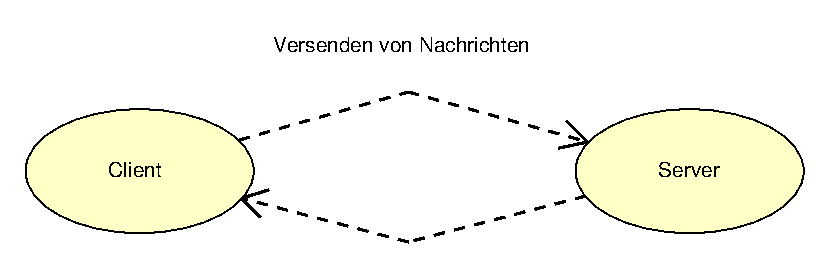
\includegraphics{images/client-server}}
	\caption{Client/Server Modell}
	\label{fig:ClientServer}
\end{figure}

\section{Prozesse und deren Rollen}

Ein verteiltes System wird anhand von Prozessen simuliert. Jeder Prozess nimmt hierbei eine oder mehrere Rollen ein. Beispielsweise kann ein Prozess die Rolle eines Clients einnehmen und ein weiterer Prozess die Rolle eines Servers. Ein Prozess kann auch Client und Server gleichzeitig sein. Es ist auch m\"{o}glich, dass ein Prozess die Rollen mehrerer Server und Clients aufeinmal einnimmt. Ob das sinnvoll ist h\"{a}ngt vom Szenario ab. Um einen Prozess zu kennzeichnen besitzt jeder Prozess eine \textbf{eindeutige} Prozess-Identifikationsnummer (PID).

\section{Nachrichten}

Damit das Client/Server Modell angewandt werden kann, m\"{u}ssen Nachrichten verschickt werden k\"{o}nnen. Eine Nachricht kann von einem Client- oder Serverprozess verschickt werden und kann beliebig viele Empf\"{a}nger haben. Der Inhalt einer Nachricht h\"{a}ngt vom verwendeten Protokoll (s.u.) ab. Um eine Nachricht zu kennzeichnen besitzt jede Nachricht eine \textbf{eindeutige} Nachrichten-Identifikationsnummer (NID).

\section{Lokale und globale Uhren}

In einer Simulation gibt es \textbf{genau eine} globale Uhr. Sie stellt die aktuelle und \textbf{immer korrekte} Zeit dar. Eine globale Uhr geht nie falsch.

Zudem besitzt jeder beteiligter Prozess eine eigene lokale Uhr. Sie stellt die aktuelle, jedoch nicht zwangsm\"{a}�ig global-korrekte, Zeit des jeweiligen Prozesses dar. Wenn die Prozesszeit nicht korrekt ist (nicht der globalen Zeit gleicht), dann wurde die Prozessuhr entweder im Laufe einer Simulation neugestellt oder sie besitzt eine Uhrabweichung. Eine Uhrabweichung gibt an, um wieviel eine Uhr falsch geht. Wenn eine lokale Uhr nicht neugesetzt wird und auch keine Uhrabweichung hat, dann gibt sie stets die korrekte globale Zeit wieder. 

\section{Ereignisse}

Eine Simulation besteht aus der Hintereinanderausf\"{u}hrung von endlich vielen Ereignissen. Beispielsweise kann es ein Ereignis geben, welches einen Prozess eine Nachricht verschicken l\"{a}�t oder den Prozess selbst abst\"{u}rzen l\"{a}�t. Jedes Ereignis tritt zu einem bestimmten Zeitpunkt ein. Wenn es zeitgleiche Ereignisse gibt, so werden sie ebenso hintereinander ausgef\"{u}hrt, behalten aber in der Simulation die selben Ausf\"{u}hrzeiten.

\section{Protokolle}

\begin{figure}[htbp]
	\centering
	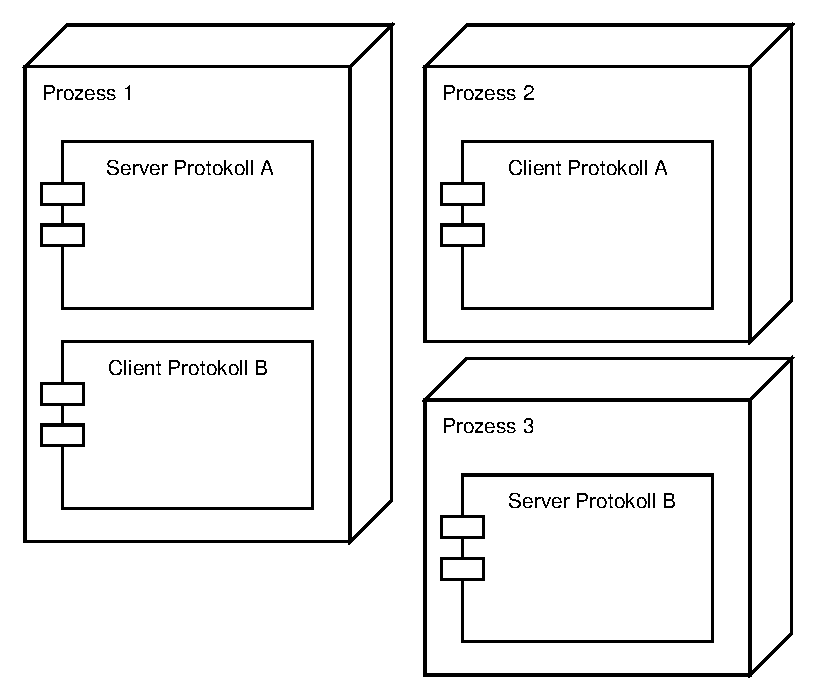
\includegraphics{images/client-server-protokolle}
	\caption{Client/Server Protokolle}
	\label{fig:ClientServerProtokolle}
\end{figure}

Eine Simulation besteht aus der Anwendung von Protokollen. Es wurde bereits erw\"{a}hnt, dass ein Prozess die Rollen von Servern und/oder Clients annehmen kann. Bei jeder Server- und Clientrolle muss zus\"{a}tzlich das dazugeh\"{o}rige Protokoll spezifiziert werden. Ein Protokoll definiert, wie ein Client und ein Server Nachrichten verschicken und wie sie bei Ankunft von Nachrichten reagieren. Ein Prozess verarbeitet eine empfangene Nachricht nur, wenn er das jeweilige Protokoll versteht.

In Abbildung \ref{fig:ClientServerProtokolle} sind 3 Prozesse dargestellt. Prozess 1 unterst\"{u}tzt serverseitig das Protokoll ``A'' und clientseitig das Protokoll ``B''. Prozess 2 unterst\"{u}tzt clientseitig das Protokoll ``A'' und Prozess 3 serverseitig das Protokoll ``B''. D.h., Prozess 1 kann mit Prozess 2 via Protokoll ``A'' und mit Prozess 3 via Protokoll ``B'' kommunizieren. Die Prozesse 2 und 3 sind zueinander inkompatibel.

\chapter{Der Simulator}

\section{Die grafische Benutzerschnittstelle}

\begin{figure}[htbp]
	\centering
	\fbox{\includegraphics{images/ss-neues-fenster-klein}}
	\caption{Der Simulator nach dem ersten Starten}
	\label{fig:NeuesFenster}
\end{figure}

Der Simulator pr\"{a}sentiert sich nach dem ersten Starten wie in Abbildung \ref{fig:NeuesFenster}. F\"{u}r die Erstellung einer neuen Simulation wird im Men\"{u} ``Datei'' (Abbildung \ref{fig:DateiMenue}) der Punkt ``Neue Simulation'' ausgew\"{a}hlt, wo anschlie�end das Einstellungsfenster f\"{u}r die neue Simulation erscheint.  Auf die einzelnen Optionen wird sp\"{a}ter genauer eingegangen und es werden nun nur die Standardeinstellungen \"{u}bernommen. Die GUI mit einer frischen Simulation sieht dann wie in Abbildung \ref{fig:NeuErstellteSimulation} aus.

\begin{figure}[htbp]
	\centering
	\fbox{\includegraphics[width=14cm]{images/ss-datei-menu}}
	\caption{Datei-Men\"{u}}
	\label{fig:DateiMenue}
\end{figure}

\subsubsection{Die Men\"{u}zeile}

Im Datei-Men\"{u} (Abbildung \ref{fig:DateiMenue}) lassen sich neue Simulationen erstellen oder die aktuell ge\"{o}ffnete Simulation schliessen. Neue Simulationen \"{o}ffnen sich standardm\"{a}�ig in einem neuen Tab. Es k\"{o}nnen allerdings auch neue Simulationsfenster, die wiederrum eigene Tabs besitzen, ge\"{o}ffnet oder geschlossen werden. In jedem Tab befindet sich eine von den Anderen vollst\"{a}ndig unabh\"{a}ngige Simulation. Es k\"{o}nnen somit beliebig viele Simulationen parallel ausgef\"{u}hrt werden. Die Men\"{u}eintr\"{a}ge ``\"{O}ffnen'', ``Speichern'' und ``Speichern unter'' dienen f\"{u}r das Laden und Speichern von Simulationen. 

\begin{figure}[htbp]
	\centering
	\fbox{\includegraphics{images/ss-neue-simulation-klein}}
	\caption{Eine neue Simulation}
	\label{fig:NeuErstellteSimulation}
\end{figure}

\"{U}ber das Editieren-Men\"{u} gelangt man zu den Simulationseinstellungen, worauf sp\"{a}ter genauer eingegangen wird. Es werden in diesem Men\"{u} auch alle beteiligten Prozesse zum Editieren aufgelistet. W\"{a}hlt man dort einen Prozess aus, dann \"{o}ffnet sich der dazugeh\"{o}rige Prozesseditor. Auf diesen wird ebenso sp\"{a}ter genauer eingegangen. Das Simulator-Men\"{u} bietet die selben Optionen wie die Toolbar, welche im n\"{a}chsten Teilkapitel beschrieben wird.

Einige Men\"{u}unterpunkte sind erst erreichbar, wenn im aktuellen Fenster bereits eine Simulation erstellt oder geladen wurde.

\subsubsection{Die Toolbar}

Oben links im Simulator befindet sich die Toolbar (Abbildung \ref{fig:Toolbar}). Die Toolbar enth\"{a}lt die Funktionen, die vom Benutzer am h\"{a}ufigsten verwendet werden.

\begin{figure}[htbp]
	\centering
	\fbox{\includegraphics[width=5cm]{images/ss-neue-simulation-toolbar}}
	\caption{Die Men\"{u}zeile inklusive Toolbar}
	\label{fig:Toolbar}
\end{figure}

Die Toolbar bietet vier verschiedene Funktionalit\"{a}ten an:

\begin{itemize}
	%\setlength{\itemsep}{-1mm}
	\item Starten der Simulation; kann nur bet\"{a}tigt werden, wenn die Simulation derzeit nicht l\"{a}uft.
	\item Pausieren der Simulation, kann nur bet\"{a}tigt werden, wenn die Simulation derzeit l\"{a}uft.
	\item Wiederholen der Simulation, kann nicht bet\"{a}tigt werden, wenn die Simulation noch nicht gestartet wurde. 
	\item Zur\"{u}cksetzen der Simulation, kann nur bet\"{a}tigt werden, wenn die Simulation pausiert wurde oder wenn die Simulation abgelaufen ist.
\end{itemize}

Die Toolbar l\"{a}sst sich auch nach Belieben repositionieren (z.B. links, rechts oder unten des Simulatorfensters). Hierf\"{u}r muss per ``Drag-n-Drop'' die ``raue Fl\"{a}che'' zur Zielposition gezogen werden.

\subsubsection{Die Visualisierung}

\begin{figure}[htbp]
	\centering
	\fbox{\includegraphics[width=14cm]{images/ss-visualisierung}}
	\caption{Visualisierung einer noch nicht gestarteten Simulation}
	\label{fig:Visualisierung}
\end{figure}

Mittig rechts in Abbildung \ref{fig:NeuErstellteSimulation} befindet sich die grafische Repr\"{a}sentation der Simulation. Die X-Achse gibt die Zeit in Millisekunden an. Unsere Demo-Simulation endet nach genau 15 Sekunden. In Abbildung \ref{fig:Visualisierung} sind 3 Prozesse (mit den PIDs 1, 2 und 3) dargestellt, die jeweils einen eigenen horizontalen schwarzen Balken besitzen. Auf diesen Prozessbalken kann der Benutzer die jeweilige lokale Prozesszeit ablesen. Die vertikale rote Linie stellt die globale Simulationszeit dar. 

Die Prozessbalken dienen auch f\"{u}r Start- und Zielpunkte von Nachrichten. Wenn beispielsweise Prozess 1 eine Nachricht zum Prozess 2 verschickt, so wird eine Linie vom einen Prozessbalken zum Anderen gezeichnet. Nachrichten, die ein Prozess an sich selbst schickt, werden nicht visualisiert. Sie werden aber im Loggfenster (mehr dazu sp\"{a}ter) protokolliert.

Eine andere M\"{o}glichkeit einen Prozesseditor aufzurufen ist ein Linksklick auf den zum Prozess geh\"{o}rigen Prozessbalken. Dies muss also nicht zwingend \"{u}ber das Simulator-Men\"{u} geschehen. Ein Rechtsklick hingegen \"{o}ffnet ein Popup-Fenster mit weiteren Auswahlm\"{o}glichkeiten (Abbildung \ref{fig:RechtsklickProzessbalken}). Ein Prozess kann \"{u}ber das Popup-Men\"{u} nur dann abst\"{u}rzen oder wiederbelebt werden, wenn die Simulation aktuell l\"{a}uft.

\begin{figure}[htbp]
	\centering
	\fbox{\includegraphics[width=8.8cm]{images/ss-rechtsklick-prozessbalken}}
	\caption{Rechtsklick auf einen Prozessbalken}
	\label{fig:RechtsklickProzessbalken}
\end{figure}

Generell kann die Anzahl der Prozesse nach belieben variieren. Die Dauer der Simulation betr\"{a}gt mindestens 5 -und maximal 120 Sekunden. Die Simulation endet erst, wenn die globale Zeit 15 Sekunden erreicht hat, und nicht, wenn eine lokale Prozesszeit die 15 Sekunden erreicht.

\subsubsection{Farbliche Differenzierung}

Farben helfen dabei die Vorg\"{a}nge einer Simulation zu deuten. Standardm\"{a}�ig werden die Prozesse (Prozessbalken) und Nachrichten mit den Farben wie in Tabelle \ref{tb:Farben} aufgelistet dargestellt. Dies sind lediglich die Standarfarben, welche man \"{u}ber die Einstellungen umkonfigurieren kann.

\begin{table}
	\fbox{
	\begin{tabular}{c|l}
		\textbf{Prozessfarbe} & \textbf{Bedeutung} \\
		\hline 
		 	Schwarz & Simulation l\"{a}uft derzeit nicht (z.B. noch nicht gestartet, abgelaufen oder\\
				& pausiert)\\
		 	Orange & Die Maus befindet sich \"{u}ber den Prozessbalken\\
		 	Rot & Der Prozess ist abgest\"{u}rzt\\
			& \\
		\textbf{Nachrichtfarbe} & \textbf{Bedeutung} \\
		\hline 
		 	Gr\"{u}n & Die Nachricht ist noch unterwegs und hat das Ziel noch nicht erreicht\\
		 	Blau & Die Nachricht hat das Ziel erfolgreich erreicht\\
		 	Rot & Die Nachricht ging verloren (entweder weil der Zielprozess abgest\"{u}rzt ist\\
				& oder weil sie unterwegs verloren ging)\\

	\end{tabular}\\
	}
	\caption{Farbliche Differenzierung von Prozessen und Nachrichten}
	\label{tb:Farben}
\end{table}

\subsubsection{Die Sidebar}

Mithilfe der Sidebar lassen sich Ereignisse von Prozessen verwalten. Ganz oben in Abbildung \ref{fig:Sidebar} ist der zu verwaltende Prozess selektiert (hier mit der PID 1). In dieser Prozessauswahl gibt es auch die M\"{o}glichkeit ``Alle Prozesse'' auszuw\"{a}hlen, womit die Ereignisse aller Prozesse gleichzeitig verwaltet werden k\"{o}nnen. Unter ``Lokale Ereignisse'' versteht man diejenigen Ereignisse, die auftreten, wenn eine bestimmte lokale Zeit des dazugeh\"{o}rigen Prozesses eingetreten ist. Die darunterliegende Ereignistabelle listet alle programmierten Ereignisse (hier noch keine vorhanden) mitsamt Eintrittszeiten sowie den PIDs auf.

\begin{figure}[htbp]
	\centering
	\fbox{\includegraphics[width=9cm]{images/ss-sidebar}}
	\caption{Die Sidebar mit leerem Ereigniseditor}
	\label{fig:Sidebar}
\end{figure}

F\"{u}r die Erstellung eines neuen Ereignisses kann der Benutzer entweder mit einem Rechtsklick auf einen Prozessbalken (Abbildung \ref{fig:RechtsklickProzessbalken}) klicken, oder unterhalb der Ereignistabelle ein Ereignis ausw\"{a}hlen (Abbildung \ref{fig:Ereignisauswahl}), im darunterliegendem Textfeld die Zeit eintragen und auf ``\"{U}bernehmen'' klicken. Beispielsweise wurden auf Abbildung \ref{fig:SidebarMitEreignissen} drei Ereignisse hinzugef\"{u}gt: Absturz nach 123ms, Wiederbelebung nach 321ms und erneuerter Absturz nach 3000ms des Prozesses mit der ID 1. 

\begin{figure}[htbp]
	\centering
	\fbox{\includegraphics[width=9cm]{images/ss-ereignisauswahl}}
	\caption{Die Ereignisauswahl via Sidebar}
	\label{fig:Ereignisauswahl}
\end{figure}

Mit einem Rechtsklick auf den Ereigniseditor lassen sich alle selektierten Ereignisse entweder kopieren oder l\"{o}schen. Die Eintr\"{a}ge der Spalten f\"{u}r die Zeit und der PID lassen sich nachtr\"{a}glich editieren. Somit besteht eine komfortable M\"{o}glichkeit bereits programmierte Ereignisse auf eine andere Zeit zu verschieben oder einem anderen Prozess zuzuweisen.

In der Sidebar gibt es neben dem Ereignis-Tab einen weiteren Tab ``Variablen''. Hinter diesem Tab verbirgt sich der Prozesseditor des aktuell ausgew\"{a}hlten Prozesses. Dort k\"{o}nnen alle Variablen des Prozesses editiert werden. Dies wird sp\"{a}ter genauer behandelt. 

\begin{figure}[htbp]
	\centering
	\fbox{\includegraphics[width=9cm]{images/ss-sidebar-mit-ereignissen}}
	\caption{Der Ereigniseditor mit 3 programmierten Ereignissen}
	\label{fig:SidebarMitEreignissen}
\end{figure}

\subsubsection{Das Loggfenster}

Das Loggfenster (Abbildung \ref{fig:NeuErstellteSimulation}, unten) protokolliert  in chronologischer Reihenfolge alle eingetroffenen Ereignisse. Auf Abbildung \ref{fig:Loggfenster} sieht man das Loggfenster nach Erstellung unserer Simulation, an welcher 3 Prozesse beteiligt sind. Am Anfang eines Loggeintrages wird stets die globale Zeit in Millisekunden protokolliert. Bei jedem Prozess wird ebenso seine lokale Zeit sowie die Lamport- und die Vektor-Zeitstempel aufgef\"{u}hrt. Letztere werden sp\"{a}ter genauer behandelt. 

\begin{figure}[htbp]
	\centering
	\fbox{\includegraphics[width=16.5cm]{images/ss-loggfenster}}
	\caption{Das Loggfenster}
	\label{fig:Loggfenster}
\end{figure}

Mit dem Deaktivieren der Checkbox ``Logging'' l\"{a}�t sich das direkte Loggen von Nachrichten tempor\"{a}r deaktivieren. Ohne aktivierter Checkbox erscheinen keine neuen Nachrichten mehr im Loggfenster. Nach Reaktivieren der Checkbox werden alle ausgelassenen Nachrichten nachtr\"{a}glich in das Fenster geschrieben. Eine Deaktivierung des Loggings kann zu verbessertem Leistungsverhalten des Simulators f\"{u}hren (z.B. kein Rucklen; ist vom verwendeten Computer, auf dem der Simulator l\"{a}uft, abh\"{a}ngig). Dieser Umstand ist der sehr langsamen Java-Implementierung der JTextArea-Klasse zu verdanken.

\"{U}ber die Checkbox ``Expertenmodus'' wird der Expertenmodus aktiviert beziehungsweise deaktiviert. 

\section{Der Expertenmodus}

\begin{figure}[htbp]
	\centering
	\fbox{\includegraphics{images/ss-simulation-expertenmodus-klein}}
	\caption{Der Simulator im Expertenmodus}
	\label{fig:SimulationExpertenmodus}
\end{figure}

Der Simulator kann in zwei verschiedenen Modi betrieben werden. Es gibt einen einfachen- und einen Expertenmodus. Der Simulator started standardm\"{a}�ig im einfachen Modus, so dass sich der Benutzer nicht mit der vollen Funktionalit\"{a}t des Simulators auf einmal auseinandersetzen mu�. Der einfache Modus ist \"{u}bersichtlicher, bietet jedoch weniger Funktionen an. Der Expertenmodus eigent sich f\"{u}r mehr erfahrene Anwender und bietet dementsprechend auch mehr Flexibilit\"{a}t. Der Expertenmodus kann \"{u}ber die gleichnamige Checkbox unterhalb des Loggfensters oder \"{u}ber die Simulationseinstellungen aktiviert oder deaktiviert werden.  Auf Abbildung \ref{fig:SimulationExpertenmodus} ist der Simulator im Expertenmodus zu sehen. Wenn man den Simulator im Expertenmodus mit Abbildung \ref{fig:NeuErstellteSimulation} vergleicht, dann fallen einige Unterschiede auf, die nun aufs Weitere behandelt werden.

\begin{figure}[htbp]
	\centering
	\fbox{\includegraphics[width=9cm]{images/ss-sidebar-expertenmodus}}
	\caption{Die Sidebar im Expertenmodus}
	\label{fig:SidebarExpertenmodus}
\end{figure}

Der erste Unterschied ist in der Sidebar erkennbar (Abbildung \ref{fig:SidebarExpertenmodus}). Dort sind nun, zus\"{a}tzlich den lokalen Ereignissen, auch globale Ereignisse editierbar.  Wie bereits erw\"{a}hnt, sind unter lokale Ereignisse diejenigen Ereignisse zu verstehen, die auftreten, wenn eine bestimmte lokale Zeit des dazugeh\"{o}rigen Prozesses eingetreten ist. Globale Ereignisse hingegen sind diejenigen Ereignisse, die auftreten, wenn eine bestimmte globale Zeit eingetreten ist. Ein globales Ereignis nimmt die globale Zeit- und ein lokales Ereignis die lokale Prozesszeit als Eintrittskriterium. Globale Ereignisse machen somit nur einen Unterschied, wenn sich die lokalen Prozesszeiten von der globalen Zeit unterscheiden.

Eine weitere neue Funktionalit\"{a}t ist die M\"{o}glichkeit einem neuzuerstellenen Ereignis direkt die PID zuzuweisen. Im einfachen Modus wurde, wenn man ein neues Ereignis erstellte, standardm\"{a}�ig immer die PID des aktuell ausgew\"{a}hlten Prozesses (in der obersten Combo-Box) verwendet. In dieser Combo-Box sollte man gegebenenfalls ``Alle Prozesse'' selektieren, damit im Ereigniseditor stets die Ereignisse aller Prozesse aufgelistet werden.

Weitere Unterschiede machen sich unterhalb des Loggfensters bemerkbar. Dort gibt es unter Anderem zwei neue Checkboxen ``Lamportzeit'' und ``Vektorzeit''.  Aktiviert man eine dieser beiden Checkboxen, dann wird die Lamport- beziehungsweise Vektorzeit in die Visualisierung dargestellt. \"{U}bersichtshalber kann der Benutzer nur jeweils eine dieser beiden Checkboxen aktivieren. Wenn die Lamportzeit-Checkbox bereits aktiviert ist und der Benutzer versucht die Vektorzeit-Checkbox zus\"{a}tzlich zu aktivieren, so wird die Lamportzeit-Checkbox automatisch deaktiviert und virce versa. 

%TODO: Lamport und Vektorzeit definieren!

Die Anti-Aliasing-Checkbox erm\"{o}glicht dem Benutzer Anti-Aliasing zu aktivieren und deaktivieren. Mit aktiviertem Anti-Aliasing werden alle Grafiken der Visualisierung gerundet dargestellt. Aus Performancegr\"{u}nden ist Anti-Aliasing standardm\"{a}�ig deaktiviert.

Je komplexer eine Simulation wird, desto un\"{u}bersichtlicher werden die Eintr\"{a}ge im Loggfenster. Hier f\"{a}llt es zunehmend schwerer die \"{U}bersicht aller Ereignisse zu behalten. Um dem entgegenzuwirken gibt es im Expertenmodus einen Loggfilter, welcher es erm\"{o}glicht nur die wesentlichen Daten aus den Loggs zu filtern. Der Loggfilter wird anhand der dazugeh\"{o}rigen Checkbox ``Filter'' aktiviert beziehungsweise deaktiviert. In der dahinterliegenden Eingabezeile kann ein regul\"{a}rer Ausdruck in Java-Syntax angegeben werden. Beispielsweise werden mit ``\texttt{PID: (1|2)}'' nur Loggzeilen angezeigt, die entweder ``\texttt{PID: 1}'' oder ``\texttt{PID: 2}'' beinhalten. Alle anderen Zeilen, beispielsweise mit ``\texttt{PID: 3}'', werden dabei nicht angezeigt. Mit aktiviertem Loggfilter werden nur die Loggzeilen angezeigt, auf die der regul\"{a}re Ausdruck passt. Der Loggfilter kann auch nachtr\"{a}glich aktiviert werden. Bereits protokollierte Ereignisse werden jedes Mal erneuert gefiltert. Der Loggfilter kann auch w\"{a}hrend einer laufenden Simulation verwendet werden. Wenn der Loggfilter deaktiviert wird, dann werden wieder alle Nachrichten (auch nachtr\"{a}glich) im Loggfenster angezeigt. 

\section{Ereignisse}

Es wird zwischen zwei verschiedenen Haupttypen von Ereignissen unterschieden: Programmierbare Ereignisse und nicht-programmierbare Ereignisse. Programmierbare Ereignisse lassen sich im Ereigniseditor editieren und deren Eintrittszeiten h\"{a}ngen von den lokalen Prozessuhren oder der globalen Uhr ab. Nicht-programmierbare Ereignisse lassen sich hingegen nicht im Ereigniseditor angeben und treten nicht aufgrund einer Uhrzeit auf sondern beispielsweise wenn eine Nachricht eintrifft.

\subsubsection{Prozessabsturz- und Wiederbelebung (programmierbar)}

Die beiden grundliegensten Ereignisse sind ``Prozessabsturz'' sowie ``Prozesswiederbelebung''. Wenn ein Prozess abgest\"{u}rzt ist, so wird sein Prozessbalken in rot dargestellt. Ein abgest\"{u}rzter Prozess kann keine weiteren Ereignisse mehr verarbeiten und, wenn er eine Nachricht empfangen sollte, geht diese verloren. Die einzige Ausnahme bildet ein Wiederbelebungsereignis. Ein abgest\"{u}rzter Prozess kann nichts, ausser wiederbelebt werden. W\"{a}hrend eines Prozessabsturzes l\"{a}uft die lokale Prozessuhr, abgesehen der Lamport- und Vektor-Uhren, wie gewohnt weiter. D.h. es k\"{o}nnte sein, dass ein Prozess einige seiner lokalen Ereignisse gar nicht ausf\"{u}hrt, da er zu den Ereigniseintrittszeiten abgest\"{u}rzt ist. Selbiges trifft nat\"{u}rlich auch auf globale Ereignisse zu. Wenn im echten Leben ein Computer abst\"{u}rzt oder abgeschaltet wird, dann l\"{a}uft dort die Hardwareuhr, unabh\"{a}ngig vom Betriebssystem, auch weiter.

\subsubsection{Aktivierung und Deaktivierung von Protokollen (programmierbar)}

Wir wissen bereits, dass ein Prozess mehrere Protokolle Client- und auch Serverseitig unterst\"{u}tzen kann. Welches Protokoll von einem Prozess unterst\"{u}tzt wird, kann der Benutzer anhand von Protokollaktivierungs- und Protokolldeaktivierungsereignissen konfigurieren. Somit besteht die M\"{o}glichkeit, dass ein gegebener Prozess ein bestimmtes Protokoll erst zu einem bestimmten Zeitpunkt unterst\"{u}tzt und gegebenenfalls ein anderes Protokoll abl\"{o}st. Jedes Protokoll kann entwender Server- oder Clientseitig aktiviert beziehungsweise deaktiviert werden. Welche Protokolle es gibt wird sp\"{a}ter behandelt.

\subsubsection{Weitere Protokollereignisse (programmierbar)}

Der Benutzer hat die Auswahl zwischen f\"{u}nf weiteren Protokollereignissen: 

\begin{itemize}
	\item Aktivierung des Clients des gegebenen Protokolls
	\item Aktivierung des Servers des gegebenen Protokolls
	\item Deaktivierung des Clients des gegebenen Protokolls
	\item Deaktivierung des Servers des gegebenen Protokolls
	\item Starten einer Client/Server-Anfrage des gegebenen Protokolls
\end{itemize}

Ob sich das Ereignis f\"{u}r das Starten einer Anfrage auf den Client oder Server bezieht, h\"{a}ngt vom verwendeten Protokoll ab. Man unterscheidet von Protokollen die Clientseitig- oder Serverseitig eine initiale Anfrage starten. Beispielsweise startet bei dem ``Ping-Pong Protokoll'' der Client- und bei dem ``Commit-Protokollen'' der Server immer die erste Anfrage. Es gibt kein Protokoll, wo Client und Server jeweils eine initiale Anfragen starten k\"{o}nnen. 

Bei allen dieser f\"{u}nf Ereignissen kann der betroffene Prozess noch beliebig andere Dinge, abh\"{a}ngig vom Protokoll, tun. Beispielsweise kann er den Inhalt der Nachricht generieren oder lokale Variablen initialisieren oder eine der lokalen Uhzeiten \"{a}ndern oder Wecker f\"{u}r ``Callback Ereignisse'' setzen (mehr dazu sp\"{a}ter).

\subsubsection{Nachrichtenempfang sowie Antwortnachrichten (nicht-programmierbar)}

Nachdem ein Prozess eine Anfragenachricht versendet hat, und ein weiterer Prozess diese Nachricht erh\"{a}lt, so \"{u}berpr\"{u}ft der Empf\"{a}ngerprozess zun\"{a}chst ob er das dazugeh\"{o}rige Protokoll versteht. Wenn es sich um eine Clientnachricht handelt, so mu� der Empf\"{a}nger ein Server sein und virce versa. Passt alles, so f\"{u}hrt der Empf\"{a}ngerprozess die vom Protokoll definierten Aktionen aus. In der Regel berechnet der Prozess einen Wert und schickt eine Antwortnachricht zur\"{u}ck. Es k\"{o}nnen aber auch beliebig andere Aktionen ausgef\"{u}hrt werden. 

\subsubsection{Callback-Ereignisse (nicht-programmierbar)}

Ein Callback-Ereignis kann von einem Protokoll ausgel\"{o}st werden. Das Protokoll setzt einen Wecker zur welcher lokalen Uhrzeit eine weitere Aktion ausgef\"{u}hrt werden soll. Zum Beispiel lassen sich hiermit Timeouts realisieren, wenn ein Protokoll eine Antwort erwartet, diese aber nicht eintrifft. Nach dem Timeout kann dann eine Anfrage erneuert verschickt werden! Es k\"{o}nnen beliebig viele Callback-Ereignisse definiert werden. Wenn sie noch nicht ausgef\"{u}hrt wurden und aufgrund eines anderen Ereignisses nicht mehr ben\"{o}tigt werden, k\"{o}nnen sie vom Protokoll auch wieder entfernt werden. Wenn ein Callback-Ereignis ausgef\"{u}hrt wird, kann es sich selbst wieder f\"{u}r eine weitere Ausf\"{u}hrung erneuert planen. So lassen sich periodisch wiedereintreffende Ereignisse realisieren. Beispielsweise verwendet das ``Reliable Multicast Protokoll'' Callback-Ereignisse, indem solange Anfragen verschickt werden, bis alle ben\"{o}tigten Antworten vorliegen.

\section{Einstellungen}

In diesem Abschnitt wird auf die m\"{o}glichen Simulationseinstellungen genauer eingegangen. Es wird zwischen drei verschiedenen Typen von Einstellungen unterschieden. Zun\"{a}chst gibt es globale Simulationseinstellungen. Diese beinhalten Variablen die f\"{u}r die gesamte Simulation gelten. Zudem hat jeder Prozess eigene lokale Einstellungen. Selbst jedes Protokoll hat f\"{u}r jeden Prozess eigene Einstellungen die editiert werden k\"{o}nnen. 

\subsection{Simulationseinstellungen}

Beim Erstellen einer neuen Simulation erscheint zun\"{a}chst das dazugeh\"{o}rige Einstellungsfenster (Abbildung \ref{fig:Simulationseinstellungen}). In der Regel reicht es, wenn man hier die Standardwerte \"{u}bernimmt. Es besteht auch die M\"{o}glichkeiten nach Erstellen einer Simulation die Einstellungen zu \"{a}ndern, indem man das Einstellungsfenster erneuert unter ``Editieren $\rightarrow$ Einstellungen'' aufruft.

\begin{figure}[htbp]
	\centering
	\fbox{\includegraphics{images/ss-simulationseinstellungen}}
	%\fbox{\includegraphics[width=11cm]{images/ss-simulationseinstellungen}}
	\caption{Das Fenster zu den Simulationseinstellungen}
	\label{fig:Simulationseinstellungen}
\end{figure}

Im Folgenden werden alle in den Simulationseinstellungen verf\"{u}gbaren Variablen beschrieben. Die Klammern geben den Typen und die Standardwerte an, in dem die Variablen vorliegen. 

\begin{itemize}
	\item \textbf{Prozesse empfangen eigene Nachrichten} \textit{(Boolean, false)}: Standardm\"{a}�ig k\"{o}nnen Prozesse aus \"{u}bersichtshalber keine Nachrichten empfangen, die sie selbst verschickt haben. Wenn diese Variable jedoch auf true gesetzt wird, dann kann ein Prozess auch auf selbst verschickte Nachrichten antworten. Die Zeit f\"{u}r das Versenden und Empfangen einer Nachricht an sich selbst betr\"{a}gt jedoch stets 0ms. Diese Variable sollte mit Vorsicht verwendet werden, da hierdurch, bedingt aus den 0ms, Endlosschleifen entstehen k\"{o}nnen. 
	\item \textbf{Mittelwerte der Nachrichtenausfallwahrscheinlichkeiten bilden} \textit{(Boolean, true)}: Jede Nachricht die verschickt wird hat, je nach Einstellungen, eine vom verschickendem Prozess abh\"{a}ngige zuf\"{a}llige Sendezeit. Wenn diese Option aktiviert ist, so wird der Mittelwert dieser Zeit vom Sende- und Empfangsprozess gebildet. Ansonsten wird stets die Sendezeit des Senderprozesses verwendet.
	\item \textbf{Expertenmodus aktivieren} \textit{(Boolean, false)}: Hier l\"{a}sst sich ebenso der Expertenmodus aktivieren oder deaktivieren.
	\item \textbf{Simulation periodisch wiederholen} \textit{(Boolean, false)}: Wenn diese Variable auf true gesetzt wird, so wird die Simulation jedes Mal nach Ablauf automatisch erneuert gestartet. 
	\item \textbf{Abspielgeschwindigkeit der Simulation} \textit{(Float, 0.5)}: Gibt den Faktor der Simulationsabspielgeschindigkeit an. Wenn als Faktor 1 gew\"{a}hlt wird, dann dauert eine simulierte Sekunde auch in echt eine Sekunde. Der Faktor 0.5 gibt somit an, dass die Simulation mit halber Echtzeitgschwindigkeit simuliert werden soll.
	\item \textbf{Anzahl der Prozesse} \textit{(Integer, 3)}: Gibt an wieviele Prozesse an der Simulation teilnehmen sollen. Wie schon erw\"{a}hnt kann man auch nachtr\"{a}glich via Rechtsklick auf den Prozessbalken den jeweiligen Prozess aus der Simulation entfernen oder weitere Prozesse hinzuf\"{u}gen.
	\item \textbf{Dauer der Simulation} \textit{(Integer, 15)}: Gibt die Dauer der Simulation in Sekunden an.
\end{itemize}

Die weiteren Einstellungen unter ``Einstellungen f\"{u}r neue Prozesse'' sowie ``Nachrichteneinstellungen f\"{u}r neue Prozesse'' geben lediglich Standardwerte an, die f\"{u}r neu zu erstellende Prozesse verwendet werden. 

\subsection{Prozess- und Protokolleinstellungen}

Jeder Prozess besitzt folgende Variablen, die entweder via dem Variablen-Tab in der Sidebar oder ``Editieren $\rightarrow$ Prozess \textit{PID}'' oder Linksklick auf den Prozessbalken editiert werden k\"{o}nnen:

\begin{itemize}
	\item \textbf{Uhrabweichung} \textit{(Float, 0.0)}: Gibt den Faktor $f$ an, um den die lokale Prozessuhr abweicht. Die Uhrabweichung wird wie folgt berechnet:
		\begin{itemize}
			\item $f := $ Der Faktor wie oben beschrieben
			\item $t := $ Aktuelle Prozesszeit in ms
			\item $t' := $ Die neu verstrichene Zeit in ms
		\end{itemize}
		Die Neue Zeit berechnet sich durch $t := t + t' * (1 + f)$. Der Faktor 0.0 besagt also, dass die Uhr keine Abweichung hat. F\"{u}r $f$ sind nur Werte $> -1.0$ erlaubt, da sonst die Prozessuhr r\"{u}ckw\"{a}rts laufen k\"{o}nnte. Bei allen anderen Werten wird der Faktor wieder automatisch auf 0.0 gesetzt. Da der Simulator intern mit Fliesskommazahlen doppelter Genauigkeit arbeitet, kann es zu kleinen, jedoch vernachl\"{a}ssigbaren, Rundungsfehlern kommen.
	\item \textbf{Prozessausfallwahrscheinlichkeit} \textit{(Integer, 0)}: Gibt eine Wahrscheinlichkeit in Prozent an, ob der gegebene Prozess w\"{a}hrend der Simulation zuf\"{a}llig abst\"{u}rzt. 
	\item \textbf{} \textit{(, )}:
	\item \textbf{} \textit{(, )}:
	\item \textbf{} \textit{(, )}:
	\item \textbf{} \textit{(, )}:
	\item \textbf{} \textit{(, )}:
	\item \textbf{} \textit{(, )}:
	\item \textbf{} \textit{(, )}:
\end{itemize}


\subsection{Einstellungen im Expertenmodus}

\section{Protokolle}

Im Folgenden werden alle bisher verf\"{u}gbaren Protokolle behandelt. Wie bereits beschrieben wird bei Protokollen zwischen Server- und Clientseite unterschieden. Server k\"{o}nnen auf Clientnachrichten, und Client auf Servernachrichten antworten. Jeder Prozess kann beliebig viele Protokolle sowohl Clientseitig als auch Serverseitig untest\"{u}tzen. Theoretisch ist es auch m\"{o}glich, dass ein Prozess f\"{u}r ein bestimmtes Protokoll gleichzeitig Server und Client ist. Der Benutzer kann auch weitere eigene Protokolle in der Programmiersprache Java mittels einer speziellen API (Application Programming Interface) erstellen. Wie eigene Protokolle erstellt werden k\"{o}nnen wird sp\"{a}ter behandelt. 

\subsection{Beispiel (Dummy) Protokoll}

Das Dummy-Protokoll dient lediglich als leeres Template f\"{u}r die Erstellung eigener Protokolle. Bei der Verwendung des Dummy-Protokolls werden bei Ereignissen lediglich Loggnachrichten ausgegeben, jedoch keine weiteren Aktionen ausgef\"{u}hrt.

\subsection{Das Ping-Pong Protokoll}

\begin{figure}[htbp]
	\centering
	\fbox{\includegraphics[width=10cm]{images/ss-protokoll-ping-pong}}
	\caption{Das Ping-Pong Protokoll}
	\label{fig:PingPongProto}
\end{figure}

Bei dem Ping-Pong Protokoll (Abbildung \ref{fig:PingPongProto}) werden zwischen zwei Prozessen, Client P1 und Server P2, st\"{a}ndig Nachrichten hin- und hergeschickt. Der Ping-Pong Client startet die erste Anfrage, worauf der Server dem Client antwortet. Auf diese Antwort wird vom Client wiederum geantwortet und so weiter. Jeder Nachricht wird ein Z\"{a}hler mitgeschickt, der bei jeder Station um eins inkrementiert- und jeweils im Loggfenster protokolliert wird. In der Simulation werden erst keine Antwortnachrichten mehr verschickt, wenn entweder eine Nachricht verloren geht, oder wenn die Simulationszeit das Ende erreicht hat. In Tabelle \ref{tb:PingPongTasks} sind alle f\"{u}r dieses Beispiel programmierten Ereignisse aufgef\"{u}hrt! Wichtig ist, dass Prozess 1 seinen Ping-Pong Client aktiviert, bevor er eine Ping-Pong Clientanfrage startet! Wenn die Eintrittszeiten f\"{u}r Aktivierung und das Starten der Anfrage identisch sind, so ordnet der Ereigniseditor diese Ereignisse automatisch in der richtigen Reihenfolge an.  Anhand diesen Beispiels ist auch erkennbar, dass die noch nicht ausgelieferte Nachrichten noch g\"{u}n eingef\"{a}rbt ist. Alle ausgelieferten Nachrichten tragen schon die Farbe Blau.

\begin{table}
	\centering
	\fbox{
	\begin{tabular}{c|c|l}
		\textbf{Zeit (ms)} & \textbf{PID} & \textbf{Ereignis} \\
		\hline 
		 	0 & 1 & Ping Pong Client aktivieren\\
		 	0 & 2 & Ping Pong Server aktivieren\\
		 	0 & 1 & Ping Pong Clientanfrage starten
	\end{tabular}
	}
	\caption{Programmierte Ping-Pong Ereignisse}
	\label{tb:PingPongTasks}
\end{table}

\begin{figure}[htbp]
	\centering
	\fbox{\includegraphics[width=10cm]{images/ss-protokoll-ping-pong-sturm}}
	\caption{Das Ping-Pong Protokoll (Sturm)}
	\label{fig:PingPongSturmProto}
\end{figure}

\"{A}ndert man die Ereignisse wie in Tabelle \ref{tb:PingPongSturmTasks} ab, so l\"{a}sst sich ein Ping-Pong Sturm realisieren. Dort wurde ein neuer Prozess 3 eingef\"{u}hrt, der als Ping-Pong Server fungiert. Als Ursache verdoppelt sich die Anzahl der kursierenden Nachrichten bei jedem Client-Server Roundtrip, da auf jede Clientnachricht stets 2 Serverantworten verschickt werden. In Abbildung \ref{fig:PingPongSturmProto} ist der resultierende Simulationsverlauf dargestellt.

\begin{table}
	\centering
	\fbox{
	\begin{tabular}{c|c|l}
		\textbf{Zeit (ms)} & \textbf{PID} & \textbf{Ereignis} \\
		\hline 
		 	0 & 1 & Ping Pong Client aktivieren\\
		 	0 & 2 & Ping Pong Server aktivieren\\
		 	0 & 3 & Ping Pong Server aktivieren\\
		 	0 & 1 & Ping Pong Clientanfrage starten
	\end{tabular}
	}
	\caption{Programmierte Ping-Pong Ereignisse (Sturm)}
	\label{tb:PingPongSturmTasks}
\end{table}

\subsection{Das Broadcast-Sturm Protokoll}

\begin{figure}[htbp]
	\centering
	\fbox{\includegraphics[width=10cm]{images/ss-protokoll-broadcast-sturm}}
	\caption{Das Broadcast-Sturm Protokoll}
	\label{fig:BroadcastSturmProto}
\end{figure}

Das Broadcast-Sturm Protokoll verh\"{a}lt sich \"{a}hnlich wie das Ping-Pong Protokoll. Der Unterschied besteht darin, dass sich das Protokoll anhand einer eindeutigen Broadcast-ID merkt, welche Nachrichten bereits verschickt wurden. Das Broadcast-Sturm Protokoll (Server- und Clientseitig) verschickt alle erhaltenen Nachrichten, sofern sie vom jeweiligen Prozess noch nicht schoneinmal verschickt wurden, erneuert. Somit l\"{a}sst sich, unter Verwendung mehrerer Prozesse (hier 6), wie auf Abbildung \ref{fig:BroadcastSturmProto}, ein Broadcast-Sturm erzeugen. P1 ist der Client und startet je eine Anfrage nach 0ms und 2500ms. Die Simulationsdauer betr\"{a}gt hier genau 5000ms. Da Client nur Servernachrichten und Server nur Clientnachrichten empfangen k\"{o}nnen, ist in dieser Simulation jeder Prozess, wie in Tabelle \ref{tb:BroadcastSturmTasks} angegeben, gleichzeitig Server und Client. 

\begin{table}
	\centering
	\fbox{
	\begin{tabular}{c|c|l}
		\textbf{Zeit (ms)} & \textbf{PID} & \textbf{Ereignis} \\
		\hline 
		 	0000 & 1 & Broadcaststurn Client aktivieren\\
		 	0000 & 2 & Broadcaststurn Client aktivieren\\
		 	0000 & 3 & Broadcaststurn Client aktivieren\\
		 	0000 & 4 & Broadcaststurn Client aktivieren\\
		 	0000 & 5 & Broadcaststurn Client aktivieren\\
		 	0000 & 6 & Broadcaststurn Client aktivieren\\
		 	0000 & 1 & Broadcaststurn Server aktivieren\\
		 	0000 & 2 & Broadcaststurn Server aktivieren\\
		 	0000 & 3 & Broadcaststurn Server aktivieren\\
		 	0000 & 4 & Broadcaststurn Server aktivieren\\
		 	0000 & 5 & Broadcaststurn Server aktivieren\\
		 	0000 & 6 & Broadcaststurn Server aktivieren\\
		 	0000 & 1 & Broadcaststurn Clientanfrage starten\\
		 	2500 & 1 & Broadcaststurn Clientanfrage starten
	\end{tabular}
	}
	\caption{Programmierte Broadcast-Sturm Ereignisse}
	\label{tb:BroadcastSturmTasks}
\end{table}

\subsection{Das Protokoll zur internen Synchronisierung in einem synchronen System}

\begin{figure}[htbp]
	\centering
	\fbox{\includegraphics[width=10cm]{images/ss-protokoll-time-sync}}
	\caption{Das Protokoll zur internen Synchronisierung}
	\label{fig:TimeSyncProto}
\end{figure}

\subsection{Christians Methode zur externen Synchronisierung}
 lsdkfjds lfjds flsjfsljsd flsdjf sldkfjsdlfkj 
 lsdkfjds lfjds flsjfsljsd flsdjf sldkfjsdlfkj 
 lsdkfjds lfjds flsjfsljsd flsdjf sldkfjsdlfkj 
 lsdkfjds lfjds flsjfsljsd flsdjf sldkfjsdlfkj 
 lsdkfjds lfjds flsjfsljsd flsdjf sldkfjsdlfkj 
 lsdkfjds lfjds flsjfsljsd flsdjf sldkfjsdlfkj 
 lsdkfjds lfjds flsjfsljsd flsdjf sldkfjsdlfkj 
 lsdkfjds lfjds flsjfsljsd flsdjf sldkfjsdlfkj 
 lsdkfjds lfjds flsjfsljsd flsdjf sldkfjsdlfkj 
 lsdkfjds lfjds flsjfsljsd flsdjf sldkfjsdlfkj 
 lsdkfjds lfjds flsjfsljsd flsdjf sldkfjsdlfkj 
 lsdkfjds lfjds flsjfsljsd flsdjf sldkfjsdlfkj 
 lsdkfjds lfjds flsjfsljsd flsdjf sldkfjsdlfkj 
 lsdkfjds lfjds flsjfsljsd flsdjf sldkfjsdlfkj 
 lsdkfjds lfjds flsjfsljsd flsdjf sldkfjsdlfkj 
 lsdkfjds lfjds flsjfsljsd flsdjf sldkfjsdlfkj 
 lsdkfjds lfjds flsjfsljsd flsdjf sldkfjsdlfkj 
 lsdkfjds lfjds flsjfsljsd flsdjf sldkfjsdlfkj 
 lsdkfjds lfjds flsjfsljsd flsdjf sldkfjsdlfkj 
 lsdkfjds lfjds flsjfsljsd flsdjf sldkfjsdlfkj 
 lsdkfjds lfjds flsjfsljsd flsdjf sldkfjsdlfkj 
 lsdkfjds lfjds flsjfsljsd flsdjf sldkfjsdlfkj 
 lsdkfjds lfjds flsjfsljsd flsdjf sldkfjsdlfkj 
 lsdkfjds lfjds flsjfsljsd flsdjf sldkfjsdlfkj 
 lsdkfjds lfjds flsjfsljsd flsdjf sldkfjsdlfkj 
 lsdkfjds lfjds flsjfsljsd flsdjf sldkfjsdlfkj 
 lsdkfjds lfjds flsjfsljsd flsdjf sldkfjsdlfkj 
 lsdkfjds lfjds flsjfsljsd flsdjf sldkfjsdlfkj 
 lsdkfjds lfjds flsjfsljsd flsdjf sldkfjsdlfkj 
 lsdkfjds lfjds flsjfsljsd flsdjf sldkfjsdlfkj 
 lsdkfjds lfjds flsjfsljsd flsdjf sldkfjsdlfkj 
 lsdkfjds lfjds flsjfsljsd flsdjf sldkfjsdlfkj 
 lsdkfjds lfjds flsjfsljsd flsdjf sldkfjsdlfkj 
 lsdkfjds lfjds flsjfsljsd flsdjf sldkfjsdlfkj 
 lsdkfjds lfjds flsjfsljsd flsdjf sldkfjsdlfkj 
 lsdkfjds lfjds flsjfsljsd flsdjf sldkfjsdlfkj 
 lsdkfjds lfjds flsjfsljsd flsdjf sldkfjsdlfkj 
 lsdkfjds lfjds flsjfsljsd flsdjf sldkfjsdlfkj 
 lsdkfjds lfjds flsjfsljsd flsdjf sldkfjsdlfkj 
 lsdkfjds lfjds flsjfsljsd flsdjf sldkfjsdlfkj 
 lsdkfjds lfjds flsjfsljsd flsdjf sldkfjsdlfkj 
 lsdkfjds lfjds flsjfsljsd flsdjf sldkfjsdlfkj 
 lsdkfjds lfjds flsjfsljsd flsdjf sldkfjsdlfkj 
 lsdkfjds lfjds flsjfsljsd flsdjf sldkfjsdlfkj 
 lsdkfjds lfjds flsjfsljsd flsdjf sldkfjsdlfkj 
 lsdkfjds lfjds flsjfsljsd flsdjf sldkfjsdlfkj 
 lsdkfjds lfjds flsjfsljsd flsdjf sldkfjsdlfkj 
 lsdkfjds lfjds flsjfsljsd flsdjf sldkfjsdlfkj 
 lsdkfjds lfjds flsjfsljsd flsdjf sldkfjsdlfkj 
 lsdkfjds lfjds flsjfsljsd flsdjf sldkfjsdlfkj 
 lsdkfjds lfjds flsjfsljsd flsdjf sldkfjsdlfkj 
 lsdkfjds lfjds flsjfsljsd flsdjf sldkfjsdlfkj 
 lsdkfjds lfjds flsjfsljsd flsdjf sldkfjsdlfkj 
 lsdkfjds lfjds flsjfsljsd flsdjf sldkfjsdlfkj 
 lsdkfjds lfjds flsjfsljsd flsdjf sldkfjsdlfkj 
 lsdkfjds lfjds flsjfsljsd flsdjf sldkfjsdlfkj 
 lsdkfjds lfjds flsjfsljsd flsdjf sldkfjsdlfkj 
 lsdkfjds lfjds flsjfsljsd flsdjf sldkfjsdlfkj 
 lsdkfjds lfjds flsjfsljsd flsdjf sldkfjsdlfkj 
 lsdkfjds lfjds flsjfsljsd flsdjf sldkfjsdlfkj 
 lsdkfjds lfjds flsjfsljsd flsdjf sldkfjsdlfkj 
 lsdkfjds lfjds flsjfsljsd flsdjf sldkfjsdlfkj 
 lsdkfjds lfjds flsjfsljsd flsdjf sldkfjsdlfkj 
 lsdkfjds lfjds flsjfsljsd flsdjf sldkfjsdlfkj 
 lsdkfjds lfjds flsjfsljsd flsdjf sldkfjsdlfkj 
 lsdkfjds lfjds flsjfsljsd flsdjf sldkfjsdlfkj 
 lsdkfjds lfjds flsjfsljsd flsdjf sldkfjsdlfkj 
 lsdkfjds lfjds flsjfsljsd flsdjf sldkfjsdlfkj 
 lsdkfjds lfjds flsjfsljsd flsdjf sldkfjsdlfkj 
 lsdkfjds lfjds flsjfsljsd flsdjf sldkfjsdlfkj 
 lsdkfjds lfjds flsjfsljsd flsdjf sldkfjsdlfkj 
 lsdkfjds lfjds flsjfsljsd flsdjf sldkfjsdlfkj 
 lsdkfjds lfjds flsjfsljsd flsdjf sldkfjsdlfkj 
 lsdkfjds lfjds flsjfsljsd flsdjf sldkfjsdlfkj 
 lsdkfjds lfjds flsjfsljsd flsdjf sldkfjsdlfkj 
 lsdkfjds lfjds flsjfsljsd flsdjf sldkfjsdlfkj 
 lsdkfjds lfjds flsjfsljsd flsdjf sldkfjsdlfkj 
 lsdkfjds lfjds flsjfsljsd flsdjf sldkfjsdlfkj 
 lsdkfjds lfjds flsjfsljsd flsdjf sldkfjsdlfkj 
 lsdkfjds lfjds flsjfsljsd flsdjf sldkfjsdlfkj 
 lsdkfjds lfjds flsjfsljsd flsdjf sldkfjsdlfkj 
 lsdkfjds lfjds flsjfsljsd flsdjf sldkfjsdlfkj 
 lsdkfjds lfjds flsjfsljsd flsdjf sldkfjsdlfkj 
 lsdkfjds lfjds flsjfsljsd flsdjf sldkfjsdlfkj 
 lsdkfjds lfjds flsjfsljsd flsdjf sldkfjsdlfkj 
 lsdkfjds lfjds flsjfsljsd flsdjf sldkfjsdlfkj 
 lsdkfjds lfjds flsjfsljsd flsdjf sldkfjsdlfkj 
 lsdkfjds lfjds flsjfsljsd flsdjf sldkfjsdlfkj 
 lsdkfjds lfjds flsjfsljsd flsdjf sldkfjsdlfkj 
 lsdkfjds lfjds flsjfsljsd flsdjf sldkfjsdlfkj 
 lsdkfjds lfjds flsjfsljsd flsdjf sldkfjsdlfkj 
 lsdkfjds lfjds flsjfsljsd flsdjf sldkfjsdlfkj 
 lsdkfjds lfjds flsjfsljsd flsdjf sldkfjsdlfkj 
 lsdkfjds lfjds flsjfsljsd flsdjf sldkfjsdlfkj 
 lsdkfjds lfjds flsjfsljsd flsdjf sldkfjsdlfkj 
 lsdkfjds lfjds flsjfsljsd flsdjf sldkfjsdlfkj 
 lsdkfjds lfjds flsjfsljsd flsdjf sldkfjsdlfkj 
 lsdkfjds lfjds flsjfsljsd flsdjf sldkfjsdlfkj 
 lsdkfjds lfjds flsjfsljsd flsdjf sldkfjsdlfkj 
 lsdkfjds lfjds flsjfsljsd flsdjf sldkfjsdlfkj 
 lsdkfjds lfjds flsjfsljsd flsdjf sldkfjsdlfkj 
 lsdkfjds lfjds flsjfsljsd flsdjf sldkfjsdlfkj 
 lsdkfjds lfjds flsjfsljsd flsdjf sldkfjsdlfkj 
 lsdkfjds lfjds flsjfsljsd flsdjf sldkfjsdlfkj 
 lsdkfjds lfjds flsjfsljsd flsdjf sldkfjsdlfkj 
 lsdkfjds lfjds flsjfsljsd flsdjf sldkfjsdlfkj 
 lsdkfjds lfjds flsjfsljsd flsdjf sldkfjsdlfkj 
 lsdkfjds lfjds flsjfsljsd flsdjf sldkfjsdlfkj 
 lsdkfjds lfjds flsjfsljsd flsdjf sldkfjsdlfkj 
 lsdkfjds lfjds flsjfsljsd flsdjf sldkfjsdlfkj 
 lsdkfjds lfjds flsjfsljsd flsdjf sldkfjsdlfkj 
 lsdkfjds lfjds flsjfsljsd flsdjf sldkfjsdlfkj 
 lsdkfjds lfjds flsjfsljsd flsdjf sldkfjsdlfkj 
 lsdkfjds lfjds flsjfsljsd flsdjf sldkfjsdlfkj 
 lsdkfjds lfjds flsjfsljsd flsdjf sldkfjsdlfkj 
 lsdkfjds lfjds flsjfsljsd flsdjf sldkfjsdlfkj 
 lsdkfjds lfjds flsjfsljsd flsdjf sldkfjsdlfkj 
 lsdkfjds lfjds flsjfsljsd flsdjf sldkfjsdlfkj 
 lsdkfjds lfjds flsjfsljsd flsdjf sldkfjsdlfkj 
 lsdkfjds lfjds flsjfsljsd flsdjf sldkfjsdlfkj 
 lsdkfjds lfjds flsjfsljsd flsdjf sldkfjsdlfkj 
 lsdkfjds lfjds flsjfsljsd flsdjf sldkfjsdlfkj 
 lsdkfjds lfjds flsjfsljsd flsdjf sldkfjsdlfkj 
 lsdkfjds lfjds flsjfsljsd flsdjf sldkfjsdlfkj 
 lsdkfjds lfjds flsjfsljsd flsdjf sldkfjsdlfkj 
 lsdkfjds lfjds flsjfsljsd flsdjf sldkfjsdlfkj 
 lsdkfjds lfjds flsjfsljsd flsdjf sldkfjsdlfkj 
 lsdkfjds lfjds flsjfsljsd flsdjf sldkfjsdlfkj 
 lsdkfjds lfjds flsjfsljsd flsdjf sldkfjsdlfkj 
 lsdkfjds lfjds flsjfsljsd flsdjf sldkfjsdlfkj 
 lsdkfjds lfjds flsjfsljsd flsdjf sldkfjsdlfkj 
 lsdkfjds lfjds flsjfsljsd flsdjf sldkfjsdlfkj 
 lsdkfjds lfjds flsjfsljsd flsdjf sldkfjsdlfkj 
 lsdkfjds lfjds flsjfsljsd flsdjf sldkfjsdlfkj 
 lsdkfjds lfjds flsjfsljsd flsdjf sldkfjsdlfkj 
 lsdkfjds lfjds flsjfsljsd flsdjf sldkfjsdlfkj 
 lsdkfjds lfjds flsjfsljsd flsdjf sldkfjsdlfkj 
 lsdkfjds lfjds flsjfsljsd flsdjf sldkfjsdlfkj 
 lsdkfjds lfjds flsjfsljsd flsdjf sldkfjsdlfkj 
 lsdkfjds lfjds flsjfsljsd flsdjf sldkfjsdlfkj 
 lsdkfjds lfjds flsjfsljsd flsdjf sldkfjsdlfkj 
 lsdkfjds lfjds flsjfsljsd flsdjf sldkfjsdlfkj 
 lsdkfjds lfjds flsjfsljsd flsdjf sldkfjsdlfkj 
 lsdkfjds lfjds flsjfsljsd flsdjf sldkfjsdlfkj 
 lsdkfjds lfjds flsjfsljsd flsdjf sldkfjsdlfkj 
 lsdkfjds lfjds flsjfsljsd flsdjf sldkfjsdlfkj 
 lsdkfjds lfjds flsjfsljsd flsdjf sldkfjsdlfkj 
 lsdkfjds lfjds flsjfsljsd flsdjf sldkfjsdlfkj 
 lsdkfjds lfjds flsjfsljsd flsdjf sldkfjsdlfkj 
 lsdkfjds lfjds flsjfsljsd flsdjf sldkfjsdlfkj 
 lsdkfjds lfjds flsjfsljsd flsdjf sldkfjsdlfkj 
 lsdkfjds lfjds flsjfsljsd flsdjf sldkfjsdlfkj 
 lsdkfjds lfjds flsjfsljsd flsdjf sldkfjsdlfkj 
 lsdkfjds lfjds flsjfsljsd flsdjf sldkfjsdlfkj 
 lsdkfjds lfjds flsjfsljsd flsdjf sldkfjsdlfkj 
 lsdkfjds lfjds flsjfsljsd flsdjf sldkfjsdlfkj 
 lsdkfjds lfjds flsjfsljsd flsdjf sldkfjsdlfkj 
 lsdkfjds lfjds flsjfsljsd flsdjf sldkfjsdlfkj 
 lsdkfjds lfjds flsjfsljsd flsdjf sldkfjsdlfkj 
 lsdkfjds lfjds flsjfsljsd flsdjf sldkfjsdlfkj 
 lsdkfjds lfjds flsjfsljsd flsdjf sldkfjsdlfkj 
 lsdkfjds lfjds flsjfsljsd flsdjf sldkfjsdlfkj 




\subsection{Berkeley Algorithmus zur internen Synchronisation}

\subsection{Das Ein-Phasen Commit Protokoll}

\subsection{Das Zwei-Phasen Commit Protokoll}

\subsection{Der ungen\"{u}gende (Basic) Multicast}

\subsection{Der zuverl\"{a}ssige (Reliable) Multicast}



\chapter{Die Implementierung}

In diesem Kapitel wird auf die Implementierung des Simulators eingegangen. Der Simulator wurde in der Programmiersprache Java entwickelt. Bei der Betrachtung der Zielgruppe wird klar, dass Java f\"{u}r die gestellte Aufgabe die geigneste Programmiersprache ist. Der Simulator ist somit auf jeder Platform verf\"{u}gbar, f\"{u}r die es die JRE (Java Runtime Environment) gibt und erstreckt sich somit \"{u}ber alle g\"{a}ngigen Betriebssysteme. Da an der Fachhochschule Aachen auch Java gelehrt wird, sollten hier die meisten Studenten auch eigene Erweiterungen, wie beispielsweise neue Protokolle, entwerfen k\"{o}nnen. Der Simulator wurde mit dem derzeit aktuellsten Java SDK (Software Development Kit) in der Version 6 (1.6) kompiliert.

\begin{table}
	\fbox{
	\begin{tabular}{l|l}
		\textbf{Paketname} & \textbf{Beschreibung} \\
		\hline 
		\textit{core} & Klassen f\"{u}r Prozesse und Nachrichten\\
		\textit{core.time} & Klassen f\"{u}r Zeitformate\\
		\textit{events} & Basisklassen f\"{u}r Ereignisse\\
		\textit{events.implementations} & Implementierungen von Ereignissen\\
		\textit{events.internal} & Implementierungen von internen Ereignissen\\
		\textit{exceptions} & Klassen f\"{u}r Fehlerbehandlungen\\
		\textit{prefs} & Klassen f\"{u}r die Einstellungen\\
		\textit{prefs.editors} & Klassen f\"{u}r die Editoren\\
		\textit{protocols} & Basisklassen f\"{u}r Protokolle\\
		\textit{protocols.implementations} & Implementierungen von Protokollen\\
		\textit{serialize} & Helferklassen f\"{u}r die Serialisierung von Simulationen\\
		\textit{simulator} & Klassen f\"{u}r die GUI und die Visualisierung\\
		\textit{utils} & Diverse Helferklassen\\
	\end{tabular}
	}
	\caption{Die Paketstruktur}
	\label{tb:Pakete}
\end{table}

Da es sonst den Rahmen sprengen w\"{u}rde, im Folgenden der komplette Quelltext nicht bis in das letzte Detail behandelt. Der Quelltext erstreckt sich n\"{a}mlich, einschlie�lich Kommentare, auf \"{u}ber 15.000 Zeilen und \"{u}ber 60 Dateien. Zudem ist die generierte Quelltext-Dokumentation (Javadoc) \"{u}ber 2MB gro�. Alle folgenden UML-Diagramme stellen aufgrund der \"{U}bersichtlichkeit lediglich die wesentlichen Dinge dar. Alle Details lassen sich im Quelltext und der dazugeh\"{o}rigen Dokumentation einsehen. Die Paketstruktur des Quelltextes ist in Tabelle \ref{tb:Pakete} in alphanumerischer Reihenfolge aufgelistet.  

\section{Programmierrichtlinien}

Die Programmierrichtlinien entsprechen in den meisten F\"{a}llen denen aus der Vorlesung \cite{OOS} und die Main-Methode befindet sich in der Klasse \textit{simulator.VSMain}. 

\begin{itemize}
	\item Alle Klassen- und Interfacenamen tragen als Prefix \textit{VS}, was f\"{u}r Verteilte Systeme steht. 
	\item Alle Quelltext-Dateien besitzen einen Header, der Informationen der verwendeten Lizenz angibt.
	\item Alle Quelltext-Dateien sind vollst\"{a}ndig mit Javadoc dokumentiert worden. Somit sind alle Klassen-, Attribute-, Methoden-, Methodenparameter- und Methodenr\"{u}ckgabewerte dokumentiert.
	\item Eine Quelltext-Datei hat eine maximale Zeilenl\"{a}nge von 80 Zeichen. Eine Ausnahme stellt die Klasse \textit{prefs.VSDefaultPrefs} dar, denn hier befinden sich auch l\"{a}ngere Texte die in Strings abgespeichert werden, wo manuelle Zeilenumbr\"{u}che wenig Sinn ergeben. 
	\item Es werden zuerst Klassen aus der Java-Standardbibliothek importiert, bevor Klassen aus dem VS-Simulator selbst importiert werden.
	\item F\"{u}r die Einr\"{u}ckung des Quelltextes wurde das Tool \textit{astyle} mit den Parametern \textit{--style=java --mode=java} verwendet. Hierbei wird eine Einr\"{u}ckungsl\"{a}nge von 4 Zeichen verwendet.
	\item Klassen- und Interfacenamen beginnen mit gro�en Buchstaben, w\"{a}hrend alle Variablen-, Methoden- und Attributnamen mit kleinen Buchstaben beginnen. Statische Variablen und Attribute sind komplett in Gro�buchstaben geschrieben.
	\item Namen abstrakter Klassen beginnen stets mit \textit{VSAbstract}.
\end{itemize}



\section{Einstellungen und Editoren}

Eine Simulation ist von einer Vielzahl von Einstellungen abh\"{a}ngig. Da auf diese Einstellungen in den weiteren Teilkapitel sets zur\"{u}ckgegriffen wird, macht es Sinn die dazugeh\"{o}rigen Klassen zuerst zu betrachten.

\subsubsection{Das Paket \textit{prefs}}

\begin{figure}[htbp]
	\centering
	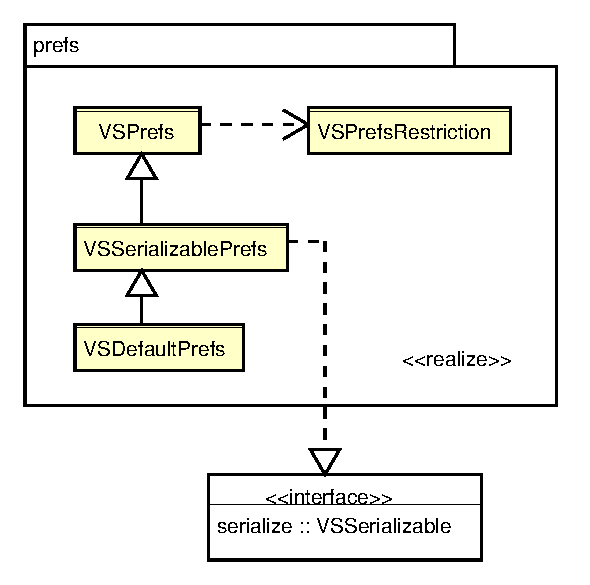
\includegraphics[width=7cm]{images/prefs}
	\caption{Das Paket \textit{prefs}}
	\label{fig:PackagePrefs}
\end{figure}

Auf Abbilung \ref{fig:PackagePrefs} ist der Aufbau des Pakets \textit{prefs} zu sehen. In einer Instanz der Klasse \textit{VSPrefs} lassen sich viele verschiedene Daten als Variablen f\"{u}r eine sp\"{a}tere Verwendung dynamisch ablegen und stellt somit einen Container f\"{u}r diese Daten dar. In einem \textit{VSPrefs}-Objekt speichert der Simulator alle seine Einstellungen ab. Zudem besitzt jedes Prozessobjekt und jedes Protokollobjekt f\"{u}r lokale Einstellungen seine eigene Instanz von \textit{VSPrefs}. Selbst Nachrichtenobjekte besitzt hiervon seine eigene Instanz, wobei hier die zu verschickenden Daten abgelegt werden k\"{o}nnen.

Jede Variable besteht aus einen Datentypen, einen Variablenamen und einer optionalen Beschreibung. Einige Datentypen unterst\"{u}tzen auch die Angabe von Minimum- und Maximumwerten (zum Beispiel besteht eine Prozentangabe aus einen Integerwert zwischen \textit{0} und \textit{100}), was mithilfe der \textit{VSPrefsRestriction}-Klasse geschieht. Da man beispielsweise bei Prozent ein \textit{\%} und bei Millisekunden ein \textit{ms} hinter der Variable sehen m\"{o}chte, kann f\"{u}r jede Variable auch ein optionaler Einheiten-String abgespeichert werden. Alle verf\"{u}gbaren Typen wurden bereits in Tabelle \ref{tb:VariablenDatentypen} aufgelistet. \textit{VSPrefs} stellt f\"{u}r alle Variablen entsprechende Zugriffsmethoden zur Verf\"{u}gung.  

Im Folgenden werden nicht alle exisierenden Methoden aufgelistet, da diese auch in der Quelltext-Dokumentation (Javadoc) eingesehen werden k\"{o}nnen. Die Methoden werden nun nur anhand des Integer-Datentyps verdeutlicht. F\"{u}r alle anderen Typen gilt fast alles analog. F\"{u}r Integer stehen in \textit{VSPrefs} folgende Methoden zur Verf\"{u}gung:

\begin{itemize}
	\setlength{\itemsep}{-2mm}
	\item \textit{void setInteger(String key, Integer val)}
	\item \textit{void setInteger(String key, Integer val, String descr)}
	\item \textit{void setInteger(String key, int val)}
	\item \textit{void setInteger(String key, int val, String descr)}
	\item \textit{Integer getIntegerObj(String key)}
	\item \textit{int getInteger(String key)}
	\item \textit{java.util.Set<String> getIntegerKeySet()}
	\item \textit{void initInteger(String key, int val) }
	\item \textit{void initInteger(String key, int val, String descr) }
	\item \textit{void initInteger(String key, int val, String descr, \\
			int minValue, int maxValue) }
	\item \textit{void initInteger(String key, int val, String descr, \\
			int minValue, int maxValue, String unit) }
	\item \textit{void initInteger(String key, int val, String descr, \\
			VSPrefsRestriction.VSIntegerPrefsRestriction r) }
	\item \textit{void initInteger(String key, int val, String descr, \\
			VSPrefsRestriction.VSIntegerPrefsRestriction r, String unit) }
\end{itemize}

Hierbei stellt \textit{key} den Variablennamen- und \textit{val} den Variablenwert dar. \textit{descr} ist eine optionale Variablenbeschreibung. Wenn f\"{u}r eine Variable keine Beschreibung existiert so wird, wie auf Abbildung \ref{fig:SimulationseinstellungenExperten} anhand der Farbvariablen schon gesehen wurde, f\"{u}r die Anzeige der Datentyp und der Variablenname verwendet. Es k\"{o}nnen sowohl Java's Integer-Objekte, als auch Java's primitiver Integer-Typ \textit{int} verwendet werden. Ein \textit{int}-Wert wird intern allerdings als Integer-Objekt abgespeichert und macht somit keinen gro�en Unterschied. Die Methode \textit{getIntegerKeySet} gibt alle vorhandenen Integer-Variablennamen (\textit{key}s) als \textit{Set} zur\"{u}ck.

\textit{VSPrefs} bietet auch eine Reihe von \textit{initInteger}-Methoden an, welche sich von den \textit{setInteger}-Methoden dadurch unterscheiden, dass sie eine Variable nur einen Wert zuweisen, wenn sie vorher noch nicht initialisiert wurde, was durch \textit{setInteger} oder \textit{initInteger} selbst geschehen sein kann. Eine komplette \"{U}bersicht aller Methoden (auch f\"{u}r andere Datentypen) gibt es in der Quelltext-Dokumentation.

\textit{VSPrefs} speichert alle Integervariablen in einem \textit{HashMap<String,Integer>}-Objekt ab, wobei der String-Wert den Variablenamen \textit{key} angibt. F\"{u}r die Beschreibung \textit{descr}, den Einheiten-String \textit{unit} sowie m\"{o}glichen Minimum- und Maximumwerte werden separate Objekte der \textit{HashMap} verwendet. Da alle \textit{HashMap}-Objekte synchronisiert sind, k\"{o}nnen alle Methoden von verschiednenen Threads gleichzeitig verwendet werden. 

Die Klasse \textit{VSDefaultPrefs} erweitert \textit{VSPrefs} und initialisiert bei Instanzierung automatisch alle verf\"{u}gbaren Simulationsvariablen mit ihren Standardwerten. Dort sind auch alle Spracheinstellungen abgelegt. Sollte jemand den Simulator in eine andere Sprache, zum Beispiel ins Englische, \"{u}bersetzen wollen, so mu� er lediglich diese Datei und die Protokoll-Klassen (mehr dazu sp\"{a}ter) editieren. Die Spracheinstellungen sind n\"{a}mlich in einem \textit{VSPrefs}--Objekt als versteckte String-Variablen abgespeichert. Versteckte Variablen werden im Editor nicht angezeigt. 

\subsubsection{Das Paket \textit{prefs.editors}}
\begin{figure}[htbp]
	\centering
	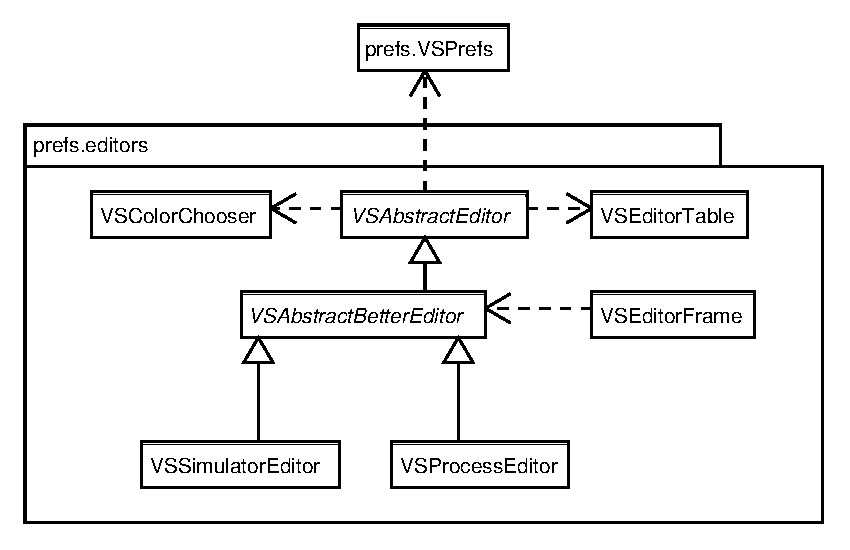
\includegraphics[width=11cm]{images/prefs-editors}
	\caption{Das Paket \textit{prefs.editors}}
	\label{fig:PackagePrefsEditors}
\end{figure}

Wie Variablen intern abgespeichert werden ist bereits bekannt. F\"{u}r das Editieren der Variablen werden Editor-Objekte verwendet. Auf Abbildung \ref{fig:PackagePrefsEditors} ist die Klassenstruktur des dazugeh\"{o}rigen Paketes \textit{prefs.editors} angegeben. 

Die Basis eines Editors stellt die abstrakte Klasse \textit{VSAbstractEditor} dar, dem ein \textit{VSPrefs} Objekt zum Editieren \"{u}bergeben wird. Ein Editor stellt alle verf\"{u}gbaren Variablen des \textit{VSPrefs}-Objektes im GUI dar und stellt gleichzeitig die M\"{o}glichkeit alle Variablen dar\"{u}ber zu editieren zur Verf\"{u}gung. F\"{u}r das Editieren von Farbwerten wird auf \textit{VSColorChooser} zur\"{u}ckgegriffen. Die Klasse \textit{VSEditorTable} ist f\"{u}r das \textit{JTable}-Objekt aus Java's Swing-Bibliothek zust\"{a}ndig, welches bei der graphischen Darstellung aller Variablen eingesetzt wird. Die abstrakte Klasse \textit{VSAbstractBetterEditor} wurde, wegen der \"{U}bersicht, als Zwischenschritt eingef\"{u}gt. 

Die Klasse \textit{VSSimulatorEditor} dient f\"{u}r das Editieren der globalen Simulationseinstellungen und \textit{VSProcessEditor} f\"{u}r das Editieren der Prozesseinstellungen sowie der dazugeh\"{o}rigen Protokollvariablen. Da diese beiden Klassen von \textit{VSAbstractBetterEditor} erben, k\"{o}nnen sie mithilfe von \textit{VSEditorFrame} in einem separaten Fenster angezeigt werden. Alternativ k\"{o}nnen die Editoren auch in der Sidebar im Tab ``Variablen'' angezeigt werden. Auf Abbildung \ref{fig:Simulationseinstellungen} wurde bereits ein \textit{VSEditorFrame} in Aktion gesehen.

F\"{u}r Protokolle gibt es keine separate Editor-Klasse, da sie bereits vom Prozesseditor aus editiert werden k\"{o}nnen. Dabei iteriert der Prozesseditor \"{u}ber alle f\"{u}r den Prozess verf\"{u}gbaren Protokollobjekte und f\"{u}gt deren Variablen zus\"{a}tzlich in den Prozesseditor ein. Somit erscheinen die Prozess- und die dazugeh\"{o}rigen Protokollvariablen im selben Editor. 

\section{Ereignisse}

F\"{u}r jedes Ereignis existiert eine dazugeh\"{o}rige Klasse, welche die auszuf\"{u}hrenden Aktionen implementiert. Eine Instanz davon wird, f\"{u}r eine sp\"{a}tere Ausf\"{u}hrung, in einem \textit{VSTask}-Objekt verpackt dem Task-Manager \"{u}bergeben. Auf den Task-Manager wird sp\"{a}ter noch genauer eingegangen. 
\begin{figure}[htbp]
	\centering
	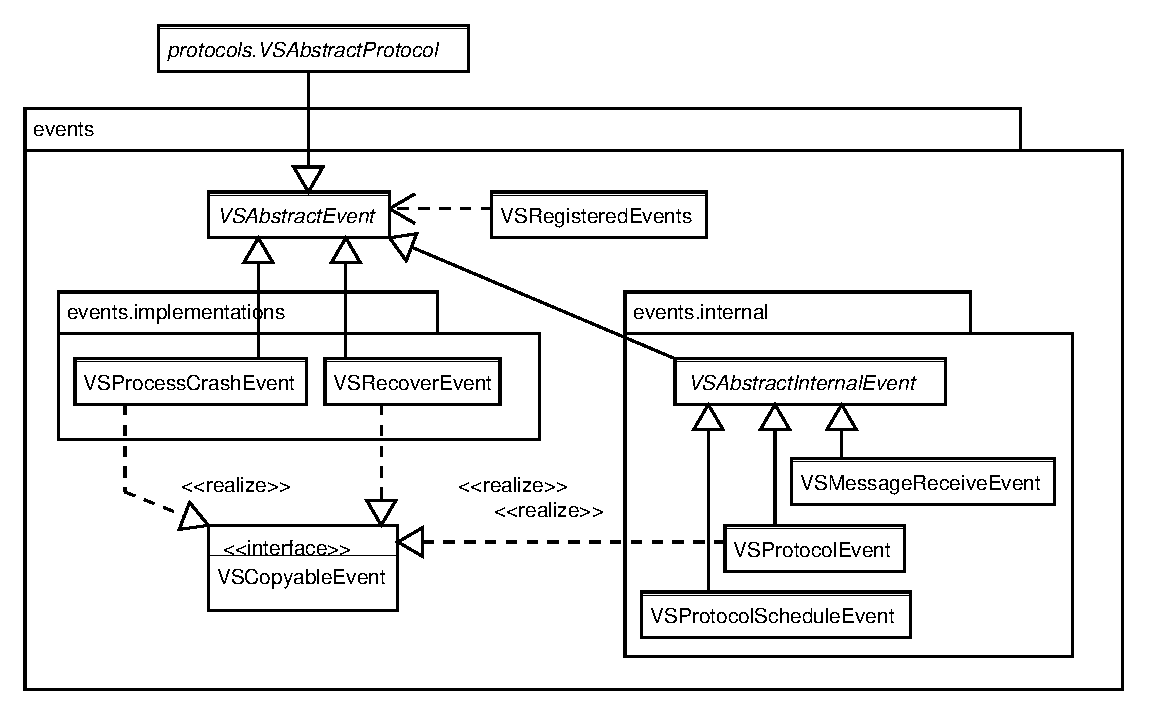
\includegraphics[width=13.5cm]{images/events}
	\caption{Die Pakete \textit{events} und \textit{events.*}}
	\label{fig:PackageEvents}
\end{figure}

Alle Ereignisklassen erweitern die abstrakte Klasse \textit{VSAbstractEvent} und m\"{u}ssen folgende Methoden implementieren:

\begin{itemize}
	\item \textit{onInit()}: Bevor ein Ereignisobjekt vom Simulator verwendet werden kann, mu� es initialisiert werden. Je nach Ereignis k\"{o}nnen hier verschiedene Werte initialisiert werden. Diese Methode wird pro Ereignisobjekt nach Erstellung nur ein einziges Mal ausgef\"{u}hrt.
	\item \textit{onStart()}: Diese Methode wird jedes Mal ausgef\"{u}hrt, wenn das Ereignis eintritt. Sie stellt somit das Kernst\"{u}ck eines Ereignisses dar. 
\end{itemize}

Jedes programmierbare Ereignis mu�, bevor es im Ereigniseditor programmiert werden kann, in der statischen Klasse \textit{VSRegisteredEvents} registriert werden. Da sich die Anzahl der verf\"{u}gbaren Ereignisse bei Laufzeit des Simulators nicht \"{a}ndert, gibt es keine Instanzen von \textit{VSRegisteredEvents}. Alle Methoden und Klassenattribute sind hier statisch. Wenn beispielsweise eigene Ereignisse implementiert werden, dann m\"{u}ssen alle neuen Ereignisse per Hand in die Datei \textit{VSRegisteredEvents.java} \"{u}bernommen- und der Simulator erneut kompiliert werden.

In der Implementierung wird zwischen drei Haupttypen von Ereignissen unterschieden, die jeweils in verschiedenen Paketen liegen:

\begin{enumerate}
	\item \textit{events.implementations}: In diesem Paket befinden sich alle Ereignisse, die ohne weitere Spezialbehanldung im Simulator eingesetzt werden k\"{o}nnen und direkt im Ereigniseditor programmierbar sind. 
		\begin{itemize}
			\item \textit{VSProcessCrashEvent}: Dieses Ereignis l\"{a}sst den dazugeh\"{o}rigen Prozess abst\"{u}rzen.
			\item \textit{VSProcessRecoverEvent}: Dieses Ereignis l\"{a}sst den dazugeh\"{o}rigen Prozess wiederbeleben.
		\end{itemize}

	\item \textit{events.internal}: In diesem Paket befinden sich alle Ereignisse, die vom Simulator intern verwendet werden und dadurch eine direkte Programmierung via Ereigniseditor ausschlie�en. 		
		\begin{itemize}
			\item \textit{VSAbstractInternalEvent}: Alle nicht-abstrakten internen Ereignisklassen erben von dieser Klasse. Sie stellt weitere Methoden zur Verf\"{u}gung, die von allen inernen Ereignissen ben\"{o}tigt werden. Derzeit betrifft dies nur Methoden zur Serialisierung der gegebenen Objekte. Auf die Serialisierung (Abspeichern/Laden) von Simulationen wird sp\"{a}ter noch genauer eingegangen.
			\item \textit{VSMessageReceiveEvent}: Diese Klasse wird f\"{u}r die Ankunft einer Nachricht bei einem Empf\"{a}ngerprozess ben\"{o}tigt. Sie kapselt die eigentliche Nachricht (ein \textit{VSMessage}-Objekt) und \"{u}berpr\"{u}ft, ob der Empf\"{a}ngerprozess das zur Nachricht dazugeh\"{o}rige Protokoll versteht. Diese Klasse \"{u}berpr\"{u}ft auch die Simulationseinstellung ``Nur relevante Nachrichten anzeigen'' und entscheidet, ob die Nachricht nach Eintreffen in der Visualisierung und im Loggfenster ber\"{u}cksichtigt werden soll oder nicht.
			\item \textit{VSProtocolEvent}: Diese Klasse implementiert gleichzeitig vier verschiedene Ereignisse: Das Aktivieren/Deaktivieren eines Servers/Clients eines gegebenen Protokolls. Der Ereigniseditor berechnet, anhand der verf\"{u}gbaren Protokolle, automatisch alle m\"{o}glichen Kombinationen und bietet sie dem Anwender in seiner Auswahl an, was auch der Grund ist weshalb sich diese Klasse in diesem Paket befindet.  F\"{u}r alle dieser vier Ereignisse wird jeweils ein Objekt von \textit{VSProtocolEvent} verwendet, jedoch mit jeweils anderen Attributwerten.  
			\item \textit{VSProtocolScheduleEvent}: Diese Klasse wird f\"{u}r die Wecker-Ereignisse ben\"{o}tigt. Wecker-Ereignisse k\"{o}nnen nur von Protokollen (mehr dazu sp\"{a}ter) erstellt werden. \textit{VSProtocolScheduleEvent} besitzt eine Referenz auf das gegebene Protokoll und ruft darauf bei Ereigniseintrittszeit entweder die Methode \textit{onServerScheduleStart} bei einem Server- oder \textit{onClientScheduleStart} bei einem Clientprotokoll auf. 
		\end{itemize}
	\item \textit{protocols.implementations}: In diesem Paket befinden sich alle Protokollimplementierung. Jedes Protokoll besitzt hier seine eigene Klasse. Alle Protokolle erben hierbei von der auf Abbildung \ref{fig:PackageEvents} zu sehenden Klasse \textit{protocols.VSAbstractProtocol}. Da \textit{protocols.VSAbstractProtocol} von \textit{events.VSAbstractEvent} erbt, kann ein Protokollobjekt auch als Ereignis eingesetzt werden. Ein solches Ereignis ruft bei Eintritt entweder die Methode \textit{onServerStart} oder die Methode \textit{onClientStart} des Protokolls auf, was einer Server- beziehungsweise einer Clientanfrage entspricht. Die Implementierung von Protokollen wird sp\"{a}ter behandelt. 
\end{enumerate}

Alle Ereignisse, die das Interface \textit{VSCopyableEvent} implementieren k\"{o}nnen im Ereigniseditor mit einem Rechtsklick kopiert werden.

\section{Prozesse, Zeitformate, Nachrichten sowie Task-Manager}

\subsubsection{Die Pakete \textit{core} und \textit{core.time}}

Das Paket \textit{core.time} auf Abbildung \ref{fig:PackageCoreTime} stellt lediglich die Klassen f\"{u}r die Vektor- und Lamportzeitstempel zur Verf\"{u}gung. F\"{u}r die normale lokale Prozesszeit wird aus Performancegr\"{u}nden keine eigene Klasse, sondern ein einfaches \textit{long}-Attribut des Prozessobjektes verwendet.

\begin{figure}[htbp]
	\centering
	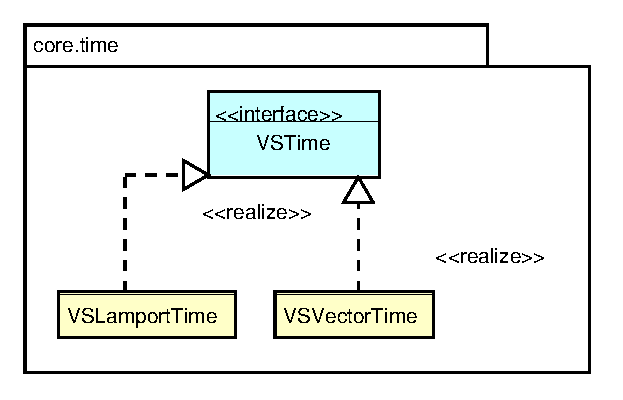
\includegraphics[width=7cm]{images/core-time}
	\caption{Das Paket \textit{core.time}}
	\label{fig:PackageCoreTime}
\end{figure}

Auf Abbildung \ref{fig:PackageCore} ist stark vereinfacht (in Wirklichkeit existieren in den angegebenen Klassen viel mehr Attribute und Methoden) das Paket \textit{core} dargestellt. Eine Simulation besteht aus einer Hintereinanderausf\"{u}hrung endlich vieler Ereignisse. F\"{u}r jedes auszuf\"{u}hrendes Ereignis wird eine Instanz von \textit{VSTask} ben\"{o}tigt, welche die Ereigniseintrittszeit als Attribut abgespeichert hat sowie eine Referenz auf das Objekt des auszuf\"{u}hrenden Ereignisses (\textit{VSAbstractEvent}) und dem Prozessobjekt besitzt. Geplante \textit{VSTask}-Instanzen werden f\"{u}r eine sp\"{a}tere Ausf\"{u}hrung dem Task-Manager \"{u}bergeben.

Die Kapselung eines \textit{VSAbstractEvent}-Objektes in einem \textit{VSTask}-Objekt erlaubt es, dass die selbe \textit{VSAbstractEvent}-Instanz mehrmals auf einmal im Task-Manager geplant werden kann. Ohne dieser Kapselung g\"{a}be es f\"{u}r jedes Ereignis lediglich nur eine einzige m\"{o}gliche Eintrittszeit. Von dieser M\"{o}glichkeit wird zum Beispiel bei den Server- und Clientanfragen eines Protokollobjektes Gebrauch gemacht. F\"{u}r jedes Protokoll kann der Anwender in einer Simulation beliebig viele Anfragen programmieren, wobei f\"{u}r jede Anfrage stets das selbe Protokollobjekt als Ereignis verwendet wird.

Jede Simulation besitzt genau eine Instanz von \textit{VSTaskManager}. Eine Instanz dieser Klasse stellt den Task-Manager dar. Er verwaltet alle \textit{VSTask}-Instanzen und \"{u}berpr\"{u}ft periodisch, ob es auszuf\"{u}hrende Ereignisse gibt. Der Task-Manager unterscheidet zwischen globalen und lokalen Ereignissen. Hierbei werden alle globalen Ereignisse (gekapselt in einem \textit{VSTask}-Objekt) in einer Priorit\"{a}ts-Warteschlange abgelegt. Die Priorit\"{a}ts-Warteschlange stellt hierbei die korrekte Ereigniseintrittsreihenfolge sicher. Da sich die lokalen Zeiten aller beteiligten Prozesse voneinander unterscheiden k\"{o}nnen, muss f\"{u}r jeden Prozess eine separate lokale Priorit\"{a}ts-Warteschlange verwendet werden, auf die jedes Prozessobjekt seine eigene Referenz hat. In den lokalen Warteschlangen sind die geplanten lokalen Ereignisse (auch gekapselt in einem \textit{VSTask}-Objekt) abgelegt. Der Task-Manager greift \"{u}ber eine \textit{java.util.ArrayList} auf alle Prozessobjekte zu und kann somit auch auf alle lokalen Warteschlangen zugreifen und diese verwalten.

\begin{figure}[htbp]
	\centering
	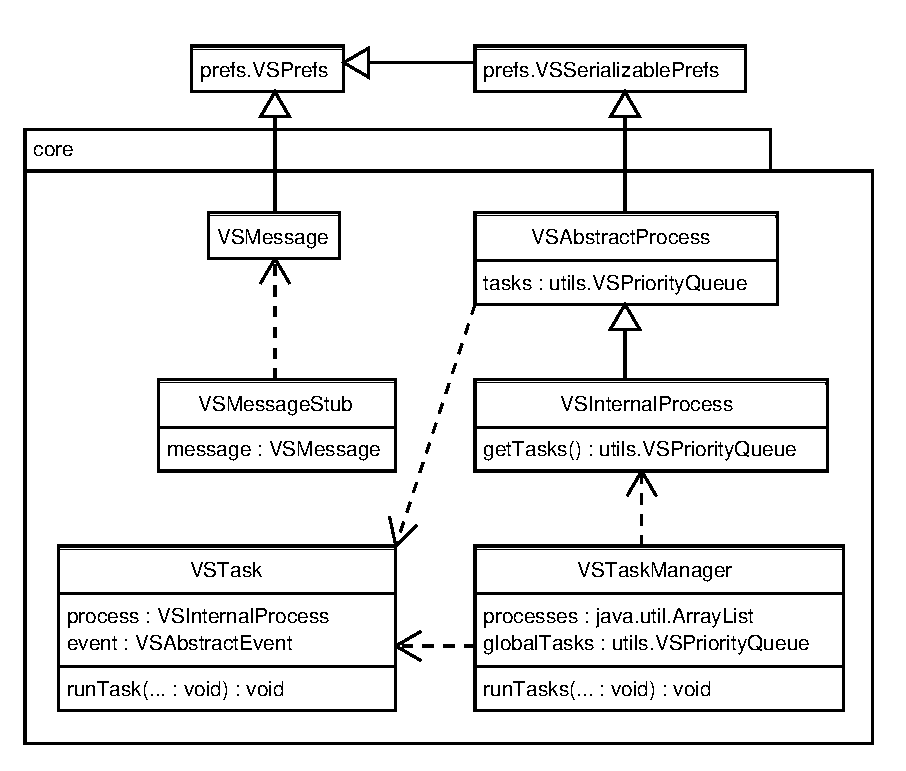
\includegraphics[width=10.0cm]{images/core}
	\caption{Das Paket \textit{core}}
	\label{fig:PackageCore}
\end{figure}

Eine Instanz von \textit{VSMessage} stellt eine Nachricht dar, die von einem Prozess verschickt wird. F\"{u}r jedes Versenden einer Nachricht wird hiervon eine Instanz gebildet, wo der Senderprozess die zu verschickende Daten ablegt. Da \textit{VSMessage} von \textit{VSPrefs} erbt, k\"{o}nnen zwischen zwei Prozessen beliebige Datentypen (Tabelle \ref{tb:VariablenDatentypen}) \"{u}ber eine Nachricht verschickt werden. Anschlie�end wird f\"{u}r jeden Empf\"{a}ngerprozess das neues Ereignisobjekt der Klasse \textit{VSMessageReceiveEvent} angelegt, welche eine Referenz der verschickten Nachricht besitzt. Danach wird ein \textit{VSTask}-Objekt instanziert, wo, wie bereits bekannt ist, die Referenz auf das Ereignisobjekt und das dazugeh\"{o}rige Prozessobjekt sowie die Ereigniseintrittszeit als Attribute gespeichert werden. Das \textit{VSTask}-Objekt wird dann dem Task-Manager "{u}bergeben, der das dazugeh\"{o}rige Ereignis ausf\"{u}hrt, wenn die Ereigniseintrittszeit eingetroffen ist. 

Via Java-Polymorphie wird das \textit{VSMessageReceiveEvent}-Objekt in ein \textit{VSAbstractEvent} umgewandelt. Die dazugeh\"{o}rige Ereigniseintrittszeit $t_e$ wird jeweils wie folgt bestimmt:

\begin{equation*}
	t_e := TODO
\end{equation*}

Erw\"{a}hnentswert ist auch die Klasse \textit{VSMessageStub}, welche ein \textit{VSMessage} kapselt. Ihr Zweck ist das Verstecken einiger Methoden von \textit{VSMessage} im Protokoll-API, welches f\"{u}r die Erstellung eigener Protokolle dient. Der Protokoll-Entwickler soll m\"{o}glichst nichts falsch machen k\"{o}nnen und deswegen soll den Protokoll-API ein eingeschr\"{a}nkter Funktionsumpfang zur Verf\"{u}rung gestellt werden. Da sich \textit{VSMessageStub} im selben Paket wie \textit{VSMessage} befindet, kann \textit{VSMessageStub} auf paket-private Methoden (diejenigen Methoden, die weder als \textit{private}, \textit{protected} noch \textit{public} gekennzeichnet sind) von \textit{VSMessage} zugreifen. Protokolle hingegen werden in einem anderen Paket implementiert und haben somit keinen Zugriff auf diese paket-privaten Methoden. Zwar kann der Protokollentwickler ein eigenes \textit{VSMessageStub}-Objekt anlegen, jedoch kann er auf diese Weise besser unterscheiden auf welche Mehhoden er zugreifen sollte und auf welche nicht. Das Protokoll-API wird sp\"{a}ter genauer behandelt. 

Der Task-Manager speichert anschlie�end die Empfangsereignisse in den lokalen Warteschlangen der Empf\"{a}ngerprozesse. Die Nachricht kommt bei einem Empf\"{a}ngerprozess an, sobald das Ereignis f\"{u}r den Empfang eintritt. F\"{u}r die korrekte Implementierung der Lamport- und Vektor-Zeitstempel wird jeder Nachricht automatisch eine Referenz der Lamport- sowie die Vektorzeit des sendenden Prozesses als Attribut beigef\"{u}gt. F\"{u}r die \"{U}berpr\"{u}fung des Protokolls wird in jeder Nachricht auch der Klassenname des jeweiligen Protokolls abgespeichert.

Eine Instanz von \textit{VSInternalProcess} repr\"{a}sentiert einen simulierten Prozess. Ein \textit{VSInternalProcess} stellt alle vom Simulator intern verwendeten Methoden zur Verf\"{u}gung, w\"{a}hrend ein \textit{VSAbstractProcess} lediglich Methoden hat, die man im Protokoll-API f\"{u}r die Erstellung eigener Protokolle verwenden darf. Da \textit{VSAbstractProcess} abstrakt ist und hiervon keine Instanz gebildet werden darf, muss stets ein \textit{VSInternalProcess}-Objekt erstellt werden. Via Polymorphie wird dieses Objekt nach \textit{VSAbstractProcess} umgewandelt und so dem Protokoll-API zur Verf\"{u}gung gestellt. 

Alle einstellbaren Prozessvariablen werden von der Klasse \textit{VSPrefs} geerbt. Aus Performancegr\"{u}nden speichert \textit{VSInternalProcess} von einigen Variablen eine lokale Kopie damit bei Neuberechnungen die Variablen nicht dauernd \"{u}ber eine \textit{HashMap} von \textit{VSPrefs} zugregriffen werden mu�. Zum Beispiel wird f\"{u}r die lokale Prozesszeit nicht auf das \textit{HashMap<String,Long>}-Objekt von \textit{VSPrefs}, sondern auf das Klassenattribut \textit{private long localTime} zugegriffen. Vor- und nach dem Editieren \"{u}ber den Prozesseditor werden die \textit{VSPrefs} beziehungsweise die lokalen Kopien auf den neusten Stand gebracht. Selbiges gilt f\"{u}r weitere Variablen wie zum Beispiel der Uhrabweichung.


\section{Protokolle}

\begin{figure}[htbp]
	\centering
	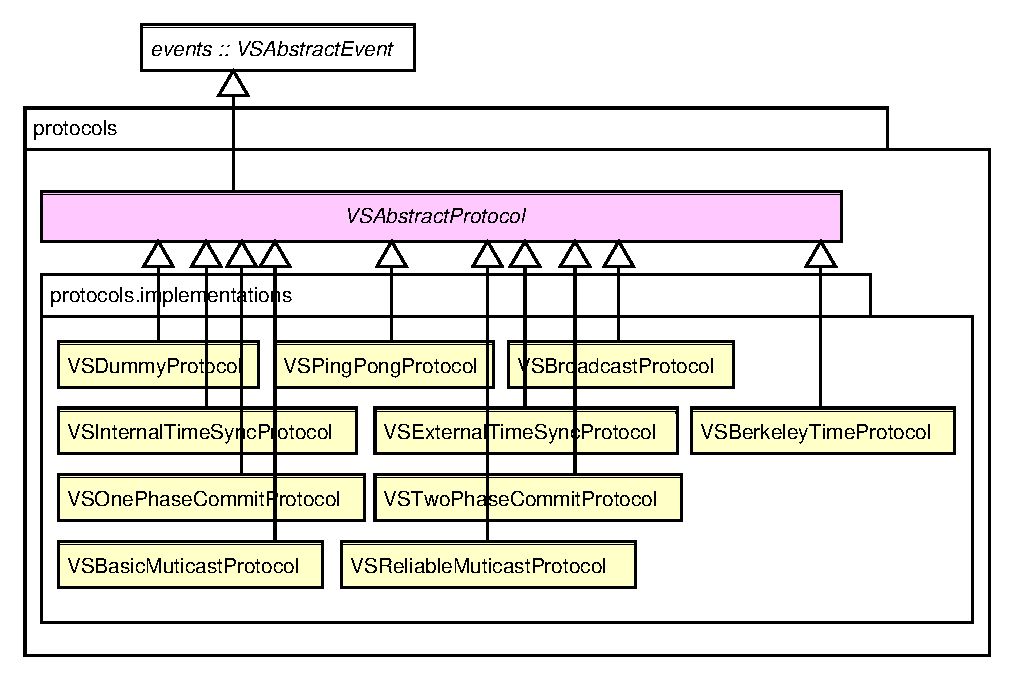
\includegraphics[width=12cm]{images/protocols}
	\caption{Die Pakete \textit{protocols} und \textit{protocols.*}}
	\label{fig:PackageProtocols}
\end{figure}

In diesem Abschnitt wird auf die Implementierung der Protokolle eingegangen. Auf Abbildung \ref{fig:PackageProtocols} sind die Pakete \textit{protocols} und \textit{protocols.implementations} dargestellt, welche f\"{u}r die Protokollimplementierungen zust\"{a}ndig sind. \textit{VSAbstractProtocol} stellt lediglich gemeinsame Methoden und Attribute zur Verf\"{u}gung, die von allen Protokollen verwendet verwenden werden k\"{o}nnen. Zus\"{a}tzlich werden von \textit{VSAbstractProtocol} die Methoden \textit{onInit()} sowie \textit{onStart()} aus der abstrakten Klasse \textit{VSAbstractEvent} implementiert, wo die jeweiligen Protokollmethoden (mit Unterscheidung zwischen Server und Client) aufgerufen werden. Jedes Protokoll hat im Paket \textit{protocols.implementations} seine eigene Klasse, die von \textit{VSAbstractProtocol} erbt. Wie bereits erw\"{a}hnt erbt \textit{VSAbstractProtocol} von \textit{VSAbstractEvent}, sodass jedes Protokoll auch als Ereignis (Server- beziehnungsweise Clientanfrage starten) eingesetzt werden kann.

Jede Protokollklasse mu� die folgenden Methoden implementieren:

\begin{itemize}
	\item Einen \"{o}ffentlichen (\textit{public}) Konstruktor. Der Konstruktor mu� angeben, ob bei dem gegebene Protokoll der Client oder der Server die Anfragen startet. 
	\item \textit{public void onClientInit()}: Bevor das Protokollobjekt benutzt werden kann, mu� es initialisiert werden. Diese Methode wird vor dem ersten Verwenden des Protokolls innerhalb einer Simulation ausgef\"{u}hrt. In der Regel werden hier Protokollvariablen unter Verwendung von \textit{VSPrefs} und Attribute der Protokollklasse initialisiert. Die hier initialisierten Protokollvariablen lassen sich vom Benutzer im Prozesseditor des jeweiligen Prozesses editieren.
	\item \textit{public void onClientReset()}: Dese Methode wird jedes Mal ausgef\"{u}hrt, wenn die Simulation zur\"{u}ckgesetzt wird.
	\item \textit{public void onClientStart()}: Diese Methode wird nur ben\"{o}tigt, wenn der Client immer die Anfragen startet. Diese Methode generiert in der Regel immer eine Clientanfrage, die via \textit{VSMessage}-Objekt an alle beteiligten Prozesse verschickt wird.
	\item \textit{public void onClientRecv(VSMessage message)}: Diese Methode wird jedes Mal Ausgef\"{u}hrt, wenn eine Servernachricht \textit{message} bei dem Client eintrifft. 
	\item \textit{public void onClientSchedule()}: Diese Methode wird jedes Mal ausgef\"{u}hrt, wenn ein Wecker-Ereignis eintritt. 
	\item \textit{public String toString()}: Diese Methode ist nur optional. Hiermit lassen sich die Loggnachrichten eines Protokolls anpassen. Wenn diese Methode in einer Protokollimplementierung ausgelassen wird, so wird stets die \textit{toString}-Methode der Mutterklasse \textit{VSAbstractProtocol} verwendet.
\end{itemize}

F\"{u}r alle hier aufgelisteten Client-Methoden sind auch die korespondierenen Server-Methoden anzugeben. Die Server-Methoden sind analog so aufgebaut wie die Client-Methoden.

\section{Serialisierung von Simulationen}

\subsection{R\"{u}ckw\"{a}rtskompatibel}

\section{Entwicklungsumgebung}

In diesem Teilkapitel soll ein kleiner Einblick in die Umgebung, mit der der Simulator entwickelt wurde, gew\"{a}hrt werden. F\"{u}r diese Diplomarbeit wurde ausschlie�lich Open Source Software verwendet. Die einzige Ausnahme stellt Microsoft Windows XP dar, worauf der Simulator auch getestet wurde. Der Simulator wurde jedoch haupts\"{a}chlich unter dem Betriebssystem FreeBSD 7.0 (\url{http://www.FreeBSD.org}), was ein open source Unix-Derivat ist, programmiert. 

Wie bereits bekannt ist, wurde Java (\url{http://java.sun.com}), was mittlerweile auch Open Source Software ist, in der Version 6 (1.6) als die Implementierungssprache gew\"{a}hlt. Als Built-Tool wurde hier auf Apache Ant gesetzt. F\"{u}r die Erstellung dieses Dokumentes wurde LaTeX verwendet.

F\"{u}r schreiben von Quelltext (Java und LaTeX) wurde GVim (\url{http://www.vim.org}) sowie Eclipse (\url{http://www.eclipse.org}) verwendet. Eclipse unterst\"{u}tzt bessere Code-Refactoring-Methoden, w\"{a}hrend GVim mit seiner Flexibilit\"{a}t und schnelleren Editierm\"{o}glichkeiten und mit Vim-Script, der eigenen Script-Engine, gl\"{a}nzt. Je nach Zweck wurde zwischen diesen beiden Umgebungen gewechselt. 

Als Versionierungssystem wurde SVN (Subversion) verwendet. F\"{u}r den Zugriff auf das SVN-Repository mittels HTTPS (Hypertext Transfer Protocol via SSL) wurde der Apache-Websever (\url{http://httpd.apache.org}) mit web\_dav-Plugin verwendet. Als SSL Zertifikat diente ein Kostenloses von CaCert (\url{http://www.CaCert.org}).

\chapter{Ausblick}

Es wurde erfolgreich ein Simulator f�r die Simulation verteilter Systeme entwickelt. Der Simulator hat bereits 10 implementierte Protokolle zur Auswahl eingebaut. Zudem steht dem Gebraucher ein sehr komfortables Protokoll-API zur Verf�gung, womit der Entwicklung neuer Protokolle quasi keine Grenzen gesetzt sind.

Dar�ber hinaus verf�gt der Simulator �ber eine Vielzahl von sehr flexiblen Einstellungsm�glichkeiten. F�r jede Simulation lassen sich somit komplett andere Konfigurationen verwenden. Jeder beteiligte Prozess hat wiederum eigene lokale Einstellungen, wo sich auch jedes Protokoll f�r jeden Prozess separat einstellen l��t. Die Anzahl und Flexibilit�t der M�glichen Szenarien wird dadurch um einen sehr gro�en Faktor erweitert.

Mit dem Ereigniseditor gibt es eine komfortable M�glichkeit eigene Szenarien zu programmieren um sie anschlie�end zu Simulieren. Hierbei kann entweder auf die bereits enthaltenen Protokolle- oder auf selbst implementierte Protokolle zugegriffen werden. Alle Dazugeh�rigen Einstellungen und programmierten Ereignisse lassen sich vom Gebraucher f�r eine sp�tere Wiederverwendung plattformunabh�ngig abspeichern. Somit k�nnen auch abgespeicherte Szenarien beispielsweise an Kommilitonen weitergegeben werden oder f�r eine sp�tere Pr�sentierung zwischengespeichert werden. Mit dem Loggfilter lassen sich mithilfe von regul�ren Ausdr�cken nur die relevanten Loggnachrichten anzeigen, was die Analyse einer Simulation erheblich vereinfacht. Weitere Funktionalit�ten wie Lamport- und Vektor-Zeitstempel sowie Anti-Aliasing runden den Simulator ab. 

Durch den objektorientierten Aufbau ist der Simulator relativ einfach erweiterbar, was nicht nur das Protokoll-API betrifft. H�tte f�r diese Diplomarbeit noch mehr Zeit zur Verf�gung gestanden, dann k�nnten einige der folgenden Funktionen (hier in alphanumerisch sortierten Reihenfolge aufgelistet) auch eingebaut worden sein:

\begin{itemize}
	\setlength{\itemsep}{-2mm}
	\item Die Simulationsdauer beliebig lang machen k�nnen. Dazu m�sste \textit{VSSimulatorVisualisation} entlang der Zeitachse scrollbar gemacht werden, sodass der Benutzer f�r eine nachtr�gliche Betrachtung des Simulationsverlaufes zu jeder beliebigen Position zur�ckspringen kann.
	\item Eine Zoomfunktion f�r die Simulationsvisualisierung einbauen.
	\item Im Ereigniseditor selbst auch periodische Ereignisse programmierbar machen. Bisher kann nur jedes Ereignis separat programmiert werden oder auf Protokoll-Interne Wecker zur�ckgegriffen werden.
	\item Lamport- und Vektor-Zeitstempel als Ereigniseintrittskriterien verwenden k�nnen.
	\item Weitere Funktionalit�ten einbauen wie zum Beispiel das Anklicken einer Nachrichtenlinie, was zu einer Nachricht alle verf�gbaren Informationen anzeigt und diese gegebenenfalls vom Benutzer editiert werden k�nnen.
	\item Tiefere Schichten des OSI-Referenzmodells simulieren k�nnen, wie zum Beispiel TCP, UDP, IP, ...
\end{itemize}

Da der Simulator h�chstwahrscheinlich unter einer Open Source Lizenz freigegeben wird, und ich mich selbst sehr f�r die Entwicklung und Anwendung von Open Source Software interessiere, werden die einen oder anderen Funktionen nachtr�glich eingebaut werden. Kommilitonen werden auch herzlich dazu eingeladen sein sich an diesem Software-Projekt zu beteiligen. Als Vorbild sei hier der CPU-Simulator M32, der von Prof. O�mann an der Fachhochschule Aachen entwickelt wurde, genannt. Hier existieren bereits einige Erweiterungen und Verbesserungen der Ursprungsversion, die von den Studenten angefertigt wurden. F�r die Entwicklung/Erweiterung wurde keine propriet�re Software verwendet, sodass jeder kostenlosen Zugriff auf die dazugeh�rigen Tools h�tte.


\appendix

\chapter{Akronyms}
\begin{acronym}
\acro{API}{Application Programming Interface}
\acro{GUI}{Graphical User Interface}
\acro{NID}{Nachrichten-Identifikationsnummer}
\acro{PID}{Prozess-Identifikationsnummer}
\acro{RTT}{Round Trip Time}
\acro{VS}{Verteiltes System}
\end{acronym}

\chapter{Akronyms}
\begin{acronym}
\acro{API}{Application Programming Interface}
\acro{GUI}{Graphical User Interface}
\acro{NID}{Nachrichten-Identifikationsnummer}
\acro{PID}{Prozess-Identifikationsnummer}
\acro{VS}{Verteiltes System}
\end{acronym}


\bibliographystyle{alpha}
\bibliography{bib/references}
%\printindex
\end{document}

%
% EOF
%

